\documentclass[journal]{IEEEtran}
\usepackage{cite}
\usepackage{amsmath,amssymb,amsfonts}
\usepackage{algorithmic}
\usepackage{graphicx}
\usepackage{textcomp}
\usepackage{xcolor}
\usepackage{booktabs}
\usepackage{multirow}
\usepackage{hyperref}
\usepackage{microtype}
\usepackage{tabularx}
\emergencystretch=2em

\begin{document}

\title{Portrait Style Transfer: A Decade Survey (2015-2025)}
\author{Feichi Chen}

\maketitle

\begin{abstract}
  Portrait Style Transfer (PST) has evolved from a niche application of texture synthesis to a cornerstone of modern generative AI, powering applications from artistic avatars to photorealistic editing. This decade-long survey (2015-2025) provides a comprehensive review of the field, systematically analyzing over 115 publications (including 28 screened arXiv preprints) and approximately 90 distinct methods across four core generative families---Optimization \& Feed-Forward Autoencoders (NST), GANs, Diffusion Models, and Autoregressive (AR) Models---plus emerging frontiers in 3D/NeRF and video stylization. To ensure rigor, our literature retrieval strategy centers on peer-reviewed venues, supplemented by 28 screened preprints from top-tier vision and graphics work, filtering for state-of-the-art mechanisms in identity-preserving stylization (see Section \ref{sec:intro:contributions} for the full search protocol). We propose a unified taxonomy based on \textit{Generative Mechanisms}, contrasting the "Structure Masters" (GANs) which historically prioritized identity preservation, with the "Texture Masters" (Diffusion Models) which offered broad stylistic diversity---though modern hybrid methods increasingly blur this boundary. Furthermore, we critically analyze the technical trade-offs between identity fidelity and stylistic abstraction---the "Uncanny Valley" of stylization---and systematically categorize solutions for geometric deformation and content-style disentanglement. Finally, we discuss emerging frontiers in video consistency and 3D-aware stylization, and summarize open challenges as a practical roadmap for future research.
\end{abstract}

\section{Introduction}
\label{sec:intro}

\IEEEPARstart{I}{n} contemporary digital media, real-time portrait editing has shifted from a niche function to a widely deployed capability. The growth of social platforms and interactive visual applications—from filters and augmented reality to live video communication—has increased demand for methods that can modify portrait appearance with both stylistic flexibility and identity consistency. This demand defines a core technical challenge for generative modeling: providing controllable portrait stylization without sacrificing speed or personal likeness.

\subsection{Technological Evolution}
\label{sec:intro:evolution}
Portrait style transfer has progressed from early texture synthesis and optimization-based neural style transfer (NST) to feed-forward stylizers, then to domain-specific GAN generators, and most recently to diffusion and autoregressive (AR) generation \cite{gatys2015ana,gatys2016image,johnson2016perceptual,ulyanov2016texture,huang2017arbitraryst,goodfellow2014generative,karras2018progressive,karras2020training,ho2020denoising,rombach_2022_cvpr}. This evolution can be interpreted as a shift in the underlying generative mechanism and its controllability: optimization-based pipelines offer direct objective control but are slow; feed-forward networks improve latency yet often lose fine control; GANs provide fast, structured portrait priors but are typically domain-constrained; diffusion models improve open-vocabulary editability but reintroduce iterative sampling cost; and AR/MLLM-related paradigms further emphasize discrete structure control and multi-modal instruction following.

\subsection{The Portrait Editing Trilemma: A Framework}
\label{sec:intro:trilemma}
In this survey, we identify a structural tension among three critical objectives. We term this the \textbf{"Portrait Editing Trilemma"}---to the best of our knowledge, the first explicit formalization of this three-way trade-off as a unifying lens for portrait editing. Its individual axes are instantiated by prior work on identity-preserving adapters \cite{wang2024instantstyle}, domain-generalizable stylization \cite{wang2025domaingp}, dual-style generation \cite{yang_2022_cvpr}, and the ArtFID fidelity metric \cite{wright2022artfidqe}:

\begin{enumerate}
  \item \textbf{Identity Preservation}: The model must rigorously maintain the subject's unique likeness throughout the editing process.
  \item \textbf{Editing Fidelity}: The model must accurately interpret and apply user instructions (typically via text prompts) to generate the desired stylistic or content changes.
  \item \textbf{Inference Speed}: The model must perform these edits in real time, ideally within a single step, to be viable for interactive applications.
\end{enumerate}

We use \textbf{Trilemma} as the primary framing in this survey; when prior work refers to an ``Impossible Triangle,'' it maps to the same three axes above.

To avoid term drift across sections, we explicitly standardize core terms in Table~\ref{tab:definitions_glossary} (Definitions/Glossary) and use these definitions consistently throughout the paper.

Existing models often sacrifice at least one of these strictly competing objectives. General-purpose editors (e.g., InstructPix2Pix~\cite{brooks2023instructpix2pix}) excel at fidelity but distort identity; specialized identity models (e.g., InstantID~\cite{wang2024instantid}) preserve likeness but often struggle with complex stylistic instructions or suffer from high latency.

Formally, let a method $m$ be characterized by its identity preservation score $I_m$, editing fidelity $E_m$, and inference speed $S_m$ (higher is better on all axes). $m$ \emph{Pareto-dominates} $m'$ if $I_m \ge I_{m'}$, $E_m \ge E_{m'}$, and $S_m \ge S_{m'}$ with at least one strict inequality. The Pareto frontier $\mathcal{P}$ is the set of non-dominated methods. Qualitatively: NST methods achieve high editing fidelity and moderate speed but weak identity; GANs offer strong identity and fast speed yet limited editing range; diffusion models attain high identity and editing fidelity at the cost of speed; AR models balance structure control and speed but introduce quantization artifacts. This mapping is formalized in the unifying framework (Section~\ref{sec:theory:unified}).

In diffusion pipelines, inference commonly uses tens of denoising steps; under typical training-free DDIM-family settings, stable stylization often falls in the 30--50 step range, while practical accelerated configurations are commonly reported around 20--50 steps \cite{song2020denoising,rombach_2022_cvpr}.

\subsection{Research Objectives and Contributions}
\label{sec:intro:contributions}
This paper makes the following principal contributions:
\begin{itemize}
  \item \textbf{Unified Mechanism Taxonomy (covering $\sim$12 NST, $\sim$25 GAN, $\sim$45 diffusion, and $\sim$10 AR methods):} We provide a systematic categorization based on the underlying generative mechanisms rather than target applications, enabling cross-paradigm comparisons.
  \item \textbf{Critical Analysis of Failure Modes}: A taxonomy of common failure patterns including identity-style conflict and texture swimming.
  \item \textbf{Evaluation Protocol}: Proposing (and calling for adoption of) a "Golden Protocol" for robust benchmarking using Multi-Pillar metrics.
\end{itemize}

\textbf{Survey Methodology:} To ensure rigorous coverage, we conducted a systematic literature search following PRISMA-inspired guidelines. Our search targeted flagship venues---CVPR, ICCV, ECCV, NeurIPS, ICLR, AAAI, ACM MM, SIGGRAPH (conferences) and TPAMI, TOG, IJCV, TVCG, TIP (journals)---published between 2015 and 2025. Keywords comprised four query categories: ``portrait stylization'', ``style transfer'', ``GAN inversion'', and ``diffusion-based editing''. The initial search returned approximately 480 records. After removing duplicates, approximately 320 unique records proceeded to title and abstract screening, which excluded purely unconditional generation, non-face stylization, and methods without explicit identity-preserving or structure-preserving controls, narrowing the pool to approximately 180 candidates. Full-text eligibility assessment yielded a final corpus of 115+ publications, comprising 88 peer-reviewed venues and 28 screened arXiv preprints. Of these, approximately 90 are distinct PST methods with dedicated stylization components; the remainder are foundational generative models (e.g., DDPM \cite{ho2020denoising}) included as theoretical prerequisites. The venue distribution spans CVPR (28), SIGGRAPH/TOG (10), ICCV (8), ECCCV (5), NeurIPS and ICLR (12), TPAMI and other journals (10), and additional conferences (15), summing to 88 peer-reviewed venues, with a further 28 arXiv preprints cited as emerging contributions. Relative to existing surveys---Kyprianidis et al.'s NPR taxonomy \cite{kyprianidis2013state}, Jing et al.'s NST survey \cite{jing2020neural}, and Xia et al.'s GAN inversion survey \cite{xia2023gan}---our work offers the first portrait-focused synthesis that bridges pre-deep-learning NPR foundations with modern generative paradigms and provides a unified evaluation protocol.

\begin{table}[t]
\centering
\caption{PRISMA-style screening funnel. Search scope: flagship venues (CVPR, ICCV, ECCV, NeurIPS, ICLR, AAAI, ACM MM, SIGGRAPH; TPAMI, TOG, IJCV, TVCG, TIP), 2015--2025; queries: \textit{portrait stylization}, \textit{style transfer}, \textit{GAN inversion}, \textit{diffusion-based editing}. Exclusion at title/abstract: purely unconditional generation, non-face stylization, and methods without explicit identity-/structure-preserving controls.}
\label{tab:prisma}
\small
\begin{tabular}{lr}
\toprule
\textbf{Screening stage} & \textbf{Records} \\
\midrule
Identified (venue + keyword search) & $\sim$480 \\
After duplicate removal & $\sim$320 \\
After title/abstract screening & $\sim$180 \\
After full-text eligibility & 115+ (88 peer-reviewed + 28 arXiv preprints) \\
\bottomrule
\end{tabular}
\end{table}

We further highlight recent one-shot and real-time portrait stylization systems as motivating use cases for the taxonomy and evaluation protocol \cite{lai2025instantportraitop,wang2024magicfacetu}. Figure~\ref{fig:teaser_trilemma} provides a visual teaser of the Trilemma framing used throughout this survey.
Unlike early diffusion frameworks that often struggle with identity preservation during abstract stylization, recent adapter-based methods improve facial-topology consistency, as discussed in Section \ref{sec:methodology}. Nevertheless, failures under large style-domain shifts remain documented in recent analyses and benchmarks \cite{wright2022artfidqe,wang2025domaingp}. Furthermore, instead of vanilla 1000-step generation, practical pipelines commonly use accelerated samplers and typically operate in about 20--50 inference steps (e.g., DDIM-family settings) \cite{song2020denoising,rombach_2022_cvpr}.

\begin{figure*}[t]
  \centering
  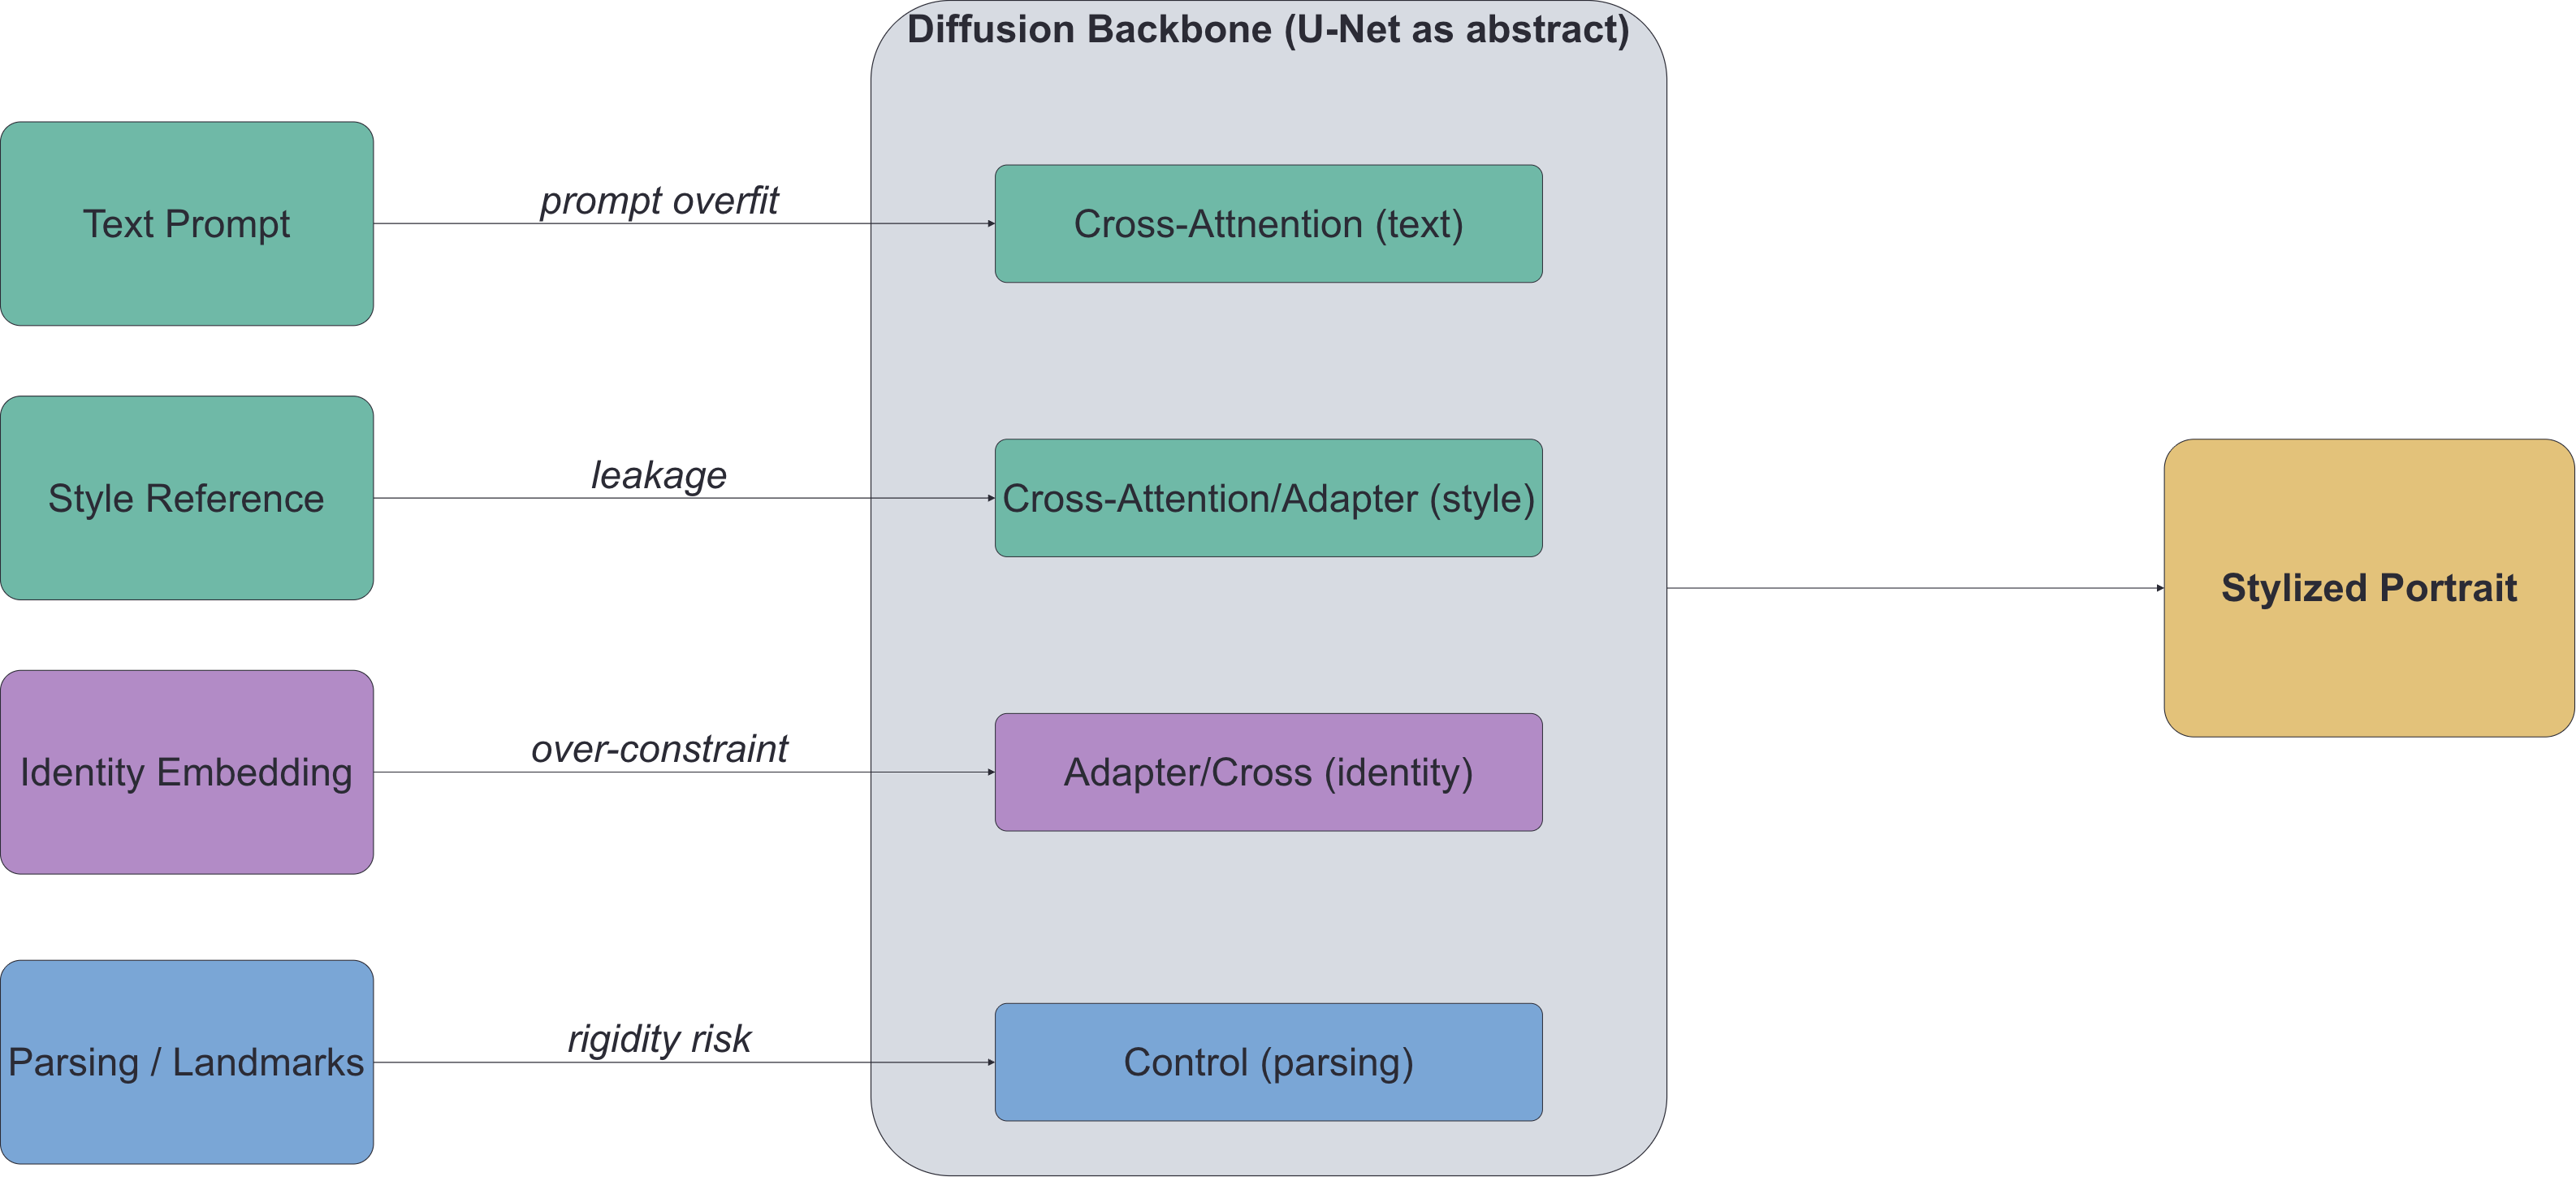
\includegraphics[width=0.98\textwidth]{images/overview.png}
  \caption{Portrait editing trilemma concept. Left: structural trade-offs among identity preservation, stylization intensity, and inference speed. Right: conceptual illustration of the Trilemma axes that frame the paradigm analysis in Section~\ref{sec:methodology}.}
  \label{fig:teaser_trilemma}
\end{figure*}

\section{Theoretical Foundations of Generative Stylization}
\label{sec:theory}

\begin{table*}[t]
  \centering
  \caption{Definitions/Glossary of core terms used in this survey.}
  \label{tab:definitions_glossary}
  \small
  \begin{tabularx}{\textwidth}{p{2.9cm}p{3.6cm}X}
    \toprule
    \textbf{Term} & \textbf{Operational meaning} & \textbf{How it is used in this survey} \\
    \midrule
    Identity & Subject-specific biometric consistency (face embedding, geometry, local traits). & Used as one Trilemma axis and the primary constraint in identity-preserving stylization. \\
    Structure & Spatial layout and semantic configuration of facial components. & Distinguished from texture to explain geometric drift and controllability limits. \\
    Geometry & Explicit shape-level facial configuration (landmarks, pose, proportions). & Treated as a stricter subset of structure when discussing deformation-heavy styles. \\
    Style Strength & Magnitude of stylistic transformation from source to target domain. & Interpreted jointly with identity metrics to diagnose under-stylization vs. over-distortion. \\
    Diversity & Variation across valid outputs under fixed content/style conditions. & Used to characterize generative breadth and mode-collapse risk. \\
    Content Leakage & Unintended transfer of source/style semantics into identity-critical regions. & Framed as a failure mode in cross-attention and entangled latent control. \\
    Temporal Consistency & Cross-frame stability of identity, texture, and motion in video stylization. & Used for evaluating flicker and drift in video-oriented PST pipelines. \\
    Texture Swimming & High-frequency texture artifacts that shift or ``swim'' across frames or spatial regions under large pose/viewpoint changes. & A failure mode diagnosed in video PST and extreme stylization settings. \\
    \bottomrule
  \end{tabularx}
\end{table*}
\subsection{Separation and Representation of Style and Identity}
\label{sec:theory:disentangle}
The primary objective of portrait style transfer (PST) can be viewed as a dual-natured optimization problem: the simultaneous preservation of semantic identity and the adoption of artistic textures. This mathematical separation of ``content'' and ``style'' is a foundational prerequisite for subsequent generative architectures, as it enables targeted manipulation of aesthetic attributes without collapsing facial structure.

This field is built on the assumption that style and content are separable in deep feature spaces. Gatys \emph{et al.} established that CNN feature statistics---specifically Gram matrices---capture style as correlations of feature maps across different layers \cite{gatys2015ana,gatys2016image}. By minimizing the distance between these correlations and a target style while maintaining feature activations for content, models achieve a rudimentary transfer. Huang and Belongie refined this idea through Adaptive Instance Normalization (AdaIN) \cite{huang2017arbitraryst}, which aligns channel-wise means and variances of content features with those of a style reference in a feed-forward manner. Linear and implicit separation strategies further formalize the notion of disentanglement between structure and texture for stylization \cite{li2018linearst,frenkel2024implicitss}. This statistical fusion can be expressed as
\begin{equation}
  Z_f = \sigma_s \left( \frac{Z_c - \mu_c}{\sigma_c} \right) + \mu_s,
\end{equation}
where $\mu_c, \sigma_c$ and $\mu_s, \sigma_s$ denote the channel-wise mean and standard deviation of the content latents $Z_c$ and style latents $Z_s$, respectively.

However, global statistics like AdaIN often fail on portraits by causing structural distortions, as they do not account for the delicate facial geometry required for human recognition. This necessitates semantic-aware representations that can protect the facial manifold while adopting complex artistic textures, including face parsing maps (as strong region-level semantic constraints), landmark sets (as sparse geometric anchors), and disentangled latent spaces in pretrained generators (e.g., StyleGAN $W/W^+$) \cite{shen2020interfacegan}. In diffusion models, a widely used working hypothesis is that self-attention primarily captures global structure while cross-attention injects conditioning signals, motivating attention-control strategies for portrait stylization \cite{hertz2023styleai, kwon2022diffuseit}.

\subsection{Loss Functions for Content--Style Disentanglement}
\label{sec:theory:losses}
Loss functions steer the trade-off between perceptual fidelity and artistic abstraction. Standard perceptual and style losses, derived from VGG-network feature maps or Gram matrices, align low-level textures. However, portraiture requires more robust semantic constraints to maintain identity, and perceptual similarity measures such as LPIPS are commonly used to quantify content deviations \cite{zhang2018lpips}.

Most portrait stylization objectives can be written as a weighted sum
\begin{equation}
  \mathcal{L}_{total} = \lambda_{sty}\mathcal{L}_{style} + \lambda_{con}\mathcal{L}_{content} + \lambda_{id}\mathcal{L}_{id} + \lambda_{geo}\mathcal{L}_{geo},
\end{equation}
where the key difference from generic NST is the explicit identity and geometry terms. Weight schedules vary substantially across architectures and normalization schemes; specific values are reported in the original method papers \cite{gatys2016image,johnson2016perceptual,huang2017arbitraryst,yang2022dualstylegan,sain2023styleface} and should not be treated as universal hyperparameters.

\subsubsection{Identity Loss}
Identity preservation is commonly enforced via face-recognition embeddings. Given a face encoder $F(\cdot)$ (e.g., ArcFace), identity loss can be defined as the cosine distance between embeddings of the source portrait $I_{src}$ and the generated output $I_{gen}$ \cite{deng2019arcface}:
\begin{equation}
  \mathcal{L}_{id} = 1 - \cos(F(I_{gen}), F(I_{src})).
\end{equation}
This constraint has become a de facto standard in portrait stylization and identity-preserving editing, especially when the target style includes strong texture changes or partial geometric deformation.

\subsubsection{Reference-free Alignment and CLIP-based Scores}
Recent work increasingly complements reference-based objectives with reference-free evaluation and guidance in joint vision--language embedding spaces. CLIPScore, for instance, measures cosine similarity between image and text (or image) embeddings, providing a robust, reference-independent proxy for how well a generated output matches the semantic concept of a target style \cite{hessel2022clipscore}.

\subsubsection{Geometric and Perceptual Losses}
To reduce structural drift, geometry-aware losses can be defined on facial landmarks. If $P(\cdot)$ extracts landmark coordinates, a simple formulation is
\begin{equation}
  \mathcal{L}_{lmk} = \sum_i \lVert P_i(I_{gen}) - P_i(I_{src}) \rVert_2.
\end{equation}
In addition, perceptual losses computed in a pretrained feature space are often used to stabilize texture transfer while maintaining plausible local details.

To prevent the ``uncanny valley'' effect, researchers further employ geometric losses such as landmark and parsing losses to stabilize facial proportions and semantic regions.

\subsection{Early Image Processing Priors}
\label{sec:theory:priors}
Modern generative models are deeply influenced by the non-parametric roots of image processing. Foundational NPR works---such as Hertzmann et al.'s Image Analogies \cite{hertzmann2001image} and Winnem\"oller et al.'s real-time video abstraction framework \cite{winnemoller2006real}---established the paradigm of example-based stylization and edge-aware filtering that later informed deep learning approaches. The broader field of image-based artistic rendering (IB-AR), surveyed by Kyprianidis et al. \cite{kyprianidis2013state}, systematizes these pre-deep-learning techniques into a taxonomy of stroke-based, region-based, and filtering-based stylization.
Early methods, such as histogram matching and Laplacian pyramids, established the methodological foundations for makeup and color transfer by decomposing images into hierarchical components \cite{chen2018facess,luan2017deepps,li2018linearst,park2019arbitraryst}.

The value of the Laplacian pyramid lies in its multi-scale decomposition, which separates high-frequency details from low-frequency structural information \cite{luan2017deepps}. This intuition can be viewed as a precursor to feature-statistics hypotheses in portrait stylization, where channel-wise means are often associated with low-frequency structure/identity and standard deviations with high-frequency texture. By establishing this logic of hierarchical feature extraction, hand-crafted techniques provided a blueprint for multi-layer modulation used in NST and later probabilistic frameworks \cite{gatys2015ana,huang2017arbitraryst}.

\subsection{Variational Autoencoders (VAEs)}
\label{sec:theory:vae}
The variational autoencoder (VAE) shifts stylization from an optimization problem to a latent-space sampling problem. By utilizing an encoder--decoder architecture regularized by a KL-divergence term, VAEs learn to map images to a structured latent manifold, enabling smooth interpolation between styles \cite{kingma2013auto}. Vector-quantized variants and specialized portrait encoders extend this idea with discrete latents for stable reconstruction and identity-aware compression \cite{esser2021vqgan,zhang2023ssrencoderes}.

VAEs, however, face a performance trade-off in portraiture: while they often capture global structure well, reconstruction objectives can oversmooth high-frequency regions (e.g., hair and eyes), leading to blurrier textures than adversarial methods. This limitation motivated the dominance of GANs for high-fidelity portrait stylization. In modern latent diffusion systems, VAEs also serve as image-to-latent compression modules for efficiency \cite{rombach_2022_cvpr}.

\subsection{Generative Adversarial Networks (GANs)}
\label{sec:theory:gan}
The adversarial paradigm introduced the photorealism and high-frequency detail required for high-quality portraiture through a min--max game between a generator $G$ and a discriminator $D$ \cite{goodfellow2014generative}. Key multi-domain translation and stabilization techniques such as StarGAN and TTUR helped generalize GAN-based stylization and improve training stability \cite{choi2018stargan,heusel2017ttur}. A critical deep dive into the StyleGAN architecture reveals that its mapping network ($Z \to W$) is a key hub for portrait control \cite{karras2019style}.

The $W$ and $W^+$ spaces enable a high degree of disentanglement, allowing independent manipulation of facial attributes (e.g., pose and expression) and artistic style. In this space, identity-critical features can be held constant while style is injected into the synthesis network. Practical StyleGAN encoders such as pSp/e4e invert real images into $W^+$ to enable image-to-image translation and editing \cite{richardson2021encoding}. For cases requiring precise reconstruction---particularly when the domain shift between source and target is large---\emph{pivotal tuning} (PTI) \cite{roich2022pivotal} extends inversion by first optimizing a latent code $w^+$ and then fine-tuning the generator:
\begin{align}
w^+ &= \arg\min_{w \in \mathcal{W}^+} \mathcal{L}_{LPIPS}\bigl(G(w), x\bigr) + \lambda_{L2}\lVert G(w) - x \rVert_2^2, \\
\min_{G'} &\;\; \lVert G'(w^+) - x \rVert_2^2 + \lambda_{LPIPS}\,\mathcal{L}_{LPIPS}\bigl(G'(w^+), x\bigr),
\end{align}
where the first stage finds a pivotal latent code and the second stage overfits the generator $G'$ to the specific portrait, trading editability for reconstruction accuracy. The reader is referred to the survey by Xia et al. \cite{xia2023gan} for a comprehensive overview of GAN inversion techniques. Despite this power, GANs struggle with one-shot transfer and domain generalization across diverse styles, which motivates the emergence of alternative continuous-time formulations \cite{karras2019style}.

\subsection{Flow Matching Models}
\label{sec:foundations:flow}
\label{sec:theory:flowmatching}
Flow-matching models provide a stable alternative to stochastic generative paths by modeling translation as an optimal-transport trajectory or a learned velocity field \cite{lipman2023flow}. Compared with noisy sampling trajectories, deterministic transport can reduce cumulative distortions and improve efficiency, and recent generalizable inverse-transport formulations connect flow matching to stylized translation and video domains \cite{cheng2023generalit,yang2023rerender}.

Recent portrait-editing systems further move from theory to practice by leveraging rectified-flow or flow-matching pipelines to avoid expensive inversion and reduce trajectory curvature. FlowEdit introduces an inversion-free ODE mapping that directly transports source portraits to edited targets under text constraints, improving structure retention for FLUX/SD3-class editors \cite{flowedit2025}. DVRF models time-dependent delta velocities to compensate oversmoothing in distilled rectified flows, helping preserve subtle facial traits such as wrinkles and skin micro-texture \cite{dvrf2025}. FlowAlign adds trajectory regularization from an optimal-control view, constraining the transport path to remain consistent with source geometry, which is particularly useful when flow-guided editing is coupled with 3D avatar stylization pipelines \cite{flowalign2025}.

In short, flow matching is no longer only a conceptual bridge between diffusion and transport; it is becoming a practical identity-preserving editor family. Its main advantage is deterministic structure control under fewer integration steps; its broader limitations are discussed in Section~\ref{sec:discussion}.

\subsection{Diffusion Models}
\label{sec:theory:diffusion}
Diffusion models formulate image generation as a gradual denoising process. The forward diffusion perturbs data $x_0 \sim p_{\text{data}}$ via a stochastic differential equation (SDE)
\begin{equation}
dx = f(x,t)\,dt + g(t)\,dw,
\end{equation}
where $f(\cdot,t)$ is the drift coefficient, $g(t)$ the diffusion coefficient, and $dw$ a Wiener process. The corresponding reverse SDE recovers the data distribution by denoising
\begin{equation}
dx = \bigl[f(x,t) - g(t)^2 \nabla_x \log p_t(x)\bigr] dt + g(t)\,d\bar{w},
\end{equation}
with $\nabla_x \log p_t(x)$ being the score function, approximated by a learned noise estimator $\epsilon_\theta(x_t,t)$ \cite{ho2020denoising,song2020denoising}. For efficient sampling, DDIM \cite{song2020denoising} proposes a deterministic reverse process
\begin{multline}
x_{t-1} = \sqrt{\alpha_{t-1}} \left( \frac{x_t - \sqrt{1-\alpha_t}\,\epsilon_\theta(x_t,t)}{\sqrt{\alpha_t}} \right) \\
+ \sqrt{1-\alpha_{t-1}}\,\epsilon_\theta(x_t,t),
\end{multline}
where $\alpha_t$ defines the noise schedule. Style conditioning is incorporated through classifier-free guidance by replacing the score estimate with $\tilde{\epsilon}_\theta(x_t,t,c) = \epsilon_\theta(x_t,t,\emptyset) + \gamma\bigl[\epsilon_\theta(x_t,t,c) - \epsilon_\theta(x_t,t,\emptyset)\bigr]$, where $c$ is the conditioning signal (e.g., style reference or text prompt) and $\gamma$ controls guidance strength.

Portrait-specific diffusion systems incorporate identity-aware constraints to avoid drift \cite{meng2021sdedit,kim2023diffface}. A key technical lever in this paradigm is \emph{attention control}: identity embeddings can be injected into cross-attention layers to stabilize identity while prompts guide texture and style \cite{wang2024instantid,zhang2023adding,ye2023ipadapter}.

Following identity-conditioned cross-attention formulations in adapter-based diffusion editors \cite{ye2023ipadapter,wang2024instantid}, one abstraction is to treat an identity embedding $e_c \in \mathbb{R}^{d_k}$ as key/value features through learned projections $W_K, W_V \in \mathbb{R}^{d_k \times d_k}$:
\begin{equation}
  \mathrm{Attn}(Q_s^i, W_K e_c, W_V e_c) =
  \mathrm{softmax}\left(\frac{Q_s^i (W_K e_c)^T}{\sqrt{d_k}}\right) W_V e_c,
\end{equation}
where $Q_s^i \in \mathbb{R}^{d_k}$ is a query feature at layer $i$ and $d_k$ is the key dimension. Following adapter alignment objectives \cite{zhang2023adding,wang2024instantid}, trainable modules can be constrained to remain close to content features using adapted query features $Q_f^i \in \mathbb{R}^{d_k}$ and content-anchored queries $Q_c^i \in \mathbb{R}^{d_k}$:
\begin{equation}
  \mathcal{L}_{align} = \frac{1}{N} \sum_{i=1}^{N} \lVert Q_f^i - Q_c^i \rVert^2.
\end{equation} In addition, following moment-matching style constraints in stylization models \cite{gatys2016image,huang2017arbitraryst}, statistic-consistency losses can encourage structure/style separation by matching moments across denoising predictions:
\begin{equation}
  \mathcal{L}_{style} =
  \lVert \mu(\epsilon_t) - \mu(\epsilon_t^c) \rVert^2
  + \lVert \sigma(\epsilon_t) - \sigma(\epsilon_t^s) \rVert^2,
\end{equation}
where $\epsilon_t$ denotes a predicted noise term and superscripts indicate conditioning sources.

Within the Adapter paradigm, the core architectures differ significantly: ControlNet utilizes spatial conditioning via residual feature injection \cite{zhang2023adding}, IP-Adapter employs decoupled cross-attention specifically for image prompts \cite{ye2023ipadapter}, and InstantID integrates ArcFace embeddings with weak spatial ControlNet conditioning \cite{wang2024instantid}.

Quantitatively, recent evaluations report competitive ArtFID scores for identity-preserving adapters such as InstantStyle \cite{wang2024instantstyle}. To ensure global artistic coherence, recent systems also employ semantic-aligned adversarial objectives that operate on pretrained vision backbones (e.g., ViT feature manifolds \cite{kwon2022diffuseit}, a diffusion-based method discussed further in Section \ref{sec:methodology}, \cite{cheng2023visual}). Despite their strengths, diffusion models typically require explicit identity/structure controls to avoid identity drift and content leakage under strong stylization.

\subsection{Unifying Framework: Control Signal, Prior, and Constraint}
\label{sec:theory:unified}

Despite their architectural diversity, all PST paradigms share a common form: a control signal $c$ encodes user intent (style, identity, or structure), a generative prior $p_\theta$ constrains the output manifold, and a constraint functional $\mathcal{L}$ drives optimization. This tripartite decomposition is expressed as
\begin{equation}
x^* = \mathcal{F}\bigl(\text{Control}(c),\; \text{Prior}(p_\theta),\; \text{Constraint}(\mathcal{L})\bigr),
\label{eq:unified}
\end{equation}
where each paradigm instantiates the three components differently (Table~\ref{tab:unified_paradigms}).

\begin{table*}[t]
\centering
\caption{Unified tripartite decomposition of PST paradigms. Each row maps the same abstract components to concrete instantiations across the four method families.}
\label{tab:unified_paradigms}
\small
\begin{tabular}{lccc}
\toprule
\textbf{Paradigm} & \textbf{Control} $(c)$ & \textbf{Prior} $(p_\theta)$ & \textbf{Constraint} $(\mathcal{L})$ \\
\midrule
NST & Style reference image & VGG feature hierarchy & Gram-matrix matching + content \\
GAN & Inverted latent $w^+$ & StyleGAN face manifold & Adversarial + identity + recon. \\
Diffusion & Text/style CLIP embedding & Score function $\nabla_x \log p_t$ & Denoising + classifier-free guidance \\
AR & Discrete visual/text tokens & Transformer next-token distrib. & Cross-entropy over codebook \\
\bottomrule
\end{tabular}
\end{table*}

\begin{table*}[t]
\centering
\caption{Qualitative mapping of PST paradigms to the Portrait Editing Trilemma axes. $\bigstar$ = strong, $\blacktriangle$ = moderate, $\bullet$ = weak.}
\label{tab:trilemma_paradigms}
\small
\begin{tabular}{lccc}
\toprule
\textbf{Paradigm} & \textbf{Identity} & \textbf{Editing Fidelity} & \textbf{Speed} \\
\midrule
NST (optimization)  & $\bullet$ & $\blacktriangle$ & $\bullet$ \\
NST (feed-forward)  & $\bullet$ & $\blacktriangle$ & $\bigstar$ \\
GAN                 & $\bigstar$ & $\blacktriangle$ & $\bigstar$ \\
Diffusion           & $\bigstar$ & $\bigstar$ & $\bullet$ \\
AR                  & $\blacktriangle$ & $\bigstar$ & $\blacktriangle$ \\
\bottomrule
\end{tabular}
\end{table*}

This decomposition reveals a clear spectrum: control signals progress from raw pixels (NST) to latent codes (GAN) to abstract embeddings (diffusion) to discrete tokens (AR); generative priors evolve from hand-crafted features to learned manifolds to score-based distributions to autoregressive distributions; and constraints transition from direct pixel objectives to learned adversarial and denoising losses. The choice of formulation determines each paradigm's inherent trade-off on the Trilemma, as detailed in Section~\ref{sec:methodology}.

\section{Methods and Method Taxonomy}
\label{sec:methodology}

We complement the paradigm-level analysis below with a qualitative capability matrix (Table~\ref{tab:comparison_matrix}) at the end of this section. Because test sets, metrics, and protocols differ across methods, direct numeric ranking would be misleading; we therefore use qualitative indicators for cross-paradigm comparisons and defer per-method numeric evidence to the original papers.

This section reviews how generative modeling frameworks have shaped portrait stylization. To provide a rigorous and symmetric analysis, we categorize the field into four foundational method families: Optimization \& Feed-Forward Autoencoders (NST), Generative Adversarial Networks (GANs), Diffusion Models, and Autoregressive (AR) Models. Following the evaluation standards, each family is systematically analyzed through its instantiation of the unifying framework (Section~\ref{sec:theory:unified}): its core generative mechanism, representative methods with coverage statistics, inherent advantages, and fundamental limitations.

To avoid ambiguity in survey writing, we use \textit{Methods and Method Taxonomy} here to denote technical model families and mechanisms, not the literature-retrieval methodology. The paper-selection and screening protocol is documented separately in the Introduction (Section~\ref{sec:intro:contributions}).

% ==========================================
% 3.1 Optimization and Feed-Forward Autoencoders (NST)
% ==========================================
\subsection{Optimization and Feed-Forward Autoencoders (NST)}
\label{sec:methodology:nst}

\textbf{Core Mechanism:} The foundational mechanism of Neural Style Transfer (NST) treats stylization as a statistical matching problem within the deep feature spaces of Convolutional Neural Networks (e.g., VGG). It explicitly separates content from style by associating spatial feature maps with structure and channel-wise statistics (e.g., Gram matrices, mean, and variance) with texture. Later extensions bypassed iterative optimization by employing feed-forward feature transformations, such as Adaptive Instance Normalization (AdaIN), which directly aligns the mean and variance of the content features to match those of the style reference.

\textbf{Representative Methods (Coverage: $\sim$12 papers):} Portrait-specific NST was first explored by Selim et al. \cite{selim2016portrait} for head portraits, following Gatys et al.'s paradigm \cite{gatys2015ana}. To achieve real-time transfer, Huang et al. introduced AdaIN \cite{huang2017arbitraryst}, which became the standard for arbitrary style transfer. For portrait-specific applications requiring dense semantic correspondences, Luan et al. proposed Deep Photo Style Transfer \cite{luan2017deepps}, while subsequent works like Avatar-Net \cite{avatar-net} and AdaAttN \cite{liu2021adaattnra} integrated attention mechanisms to decorate semantic features locally without distorting facial layouts. For a comprehensive treatment of the broader NST landscape, including pre-deep-learning foundations, we refer to the survey by Jing et al. \cite{jing2020neural}. Beyond classical optimization-based NST, feed-forward variants also explore flow-based bijective formulations for unbiased transfer \cite{artflow}, as well as multimodal unsupervised image-to-image translation that supports diverse stylized outputs from a single content image \cite{huang2018multimodal}. Puff-Net~\cite{zheng2024puffnet} further pursues efficient 2D NST through pure content--style feature fusion.

\textbf{Advantages:} These methods are highly efficient (in their feed-forward variants) and capable of achieving zero-shot arbitrary style transfer without the need for extensive domain-specific pretraining. They mathematically guarantee the decoupling of structure and texture statistics.

\textbf{Limitations:} The primary failure mode is \textit{structural drift}. Since Gram matrices and global statistics are completely agnostic to spatial geometry, these methods often misalign facial components (e.g., applying eye makeup textures to the background). Furthermore, feed-forward transforms often blur high-frequency details, resulting in "washed-out" portrait textures. Quantitatively, classic NST approaches exhibit a notable distributional gap under ArtFID---for instance, AdaIN yields an ArtFID of $13.222 \pm 0.549$ (Wright and Ommer, Table~1; Places365/COCO content with WikiArt/BAM style at $512\times512$) \cite{wright2022artfidqe}---relative to diffusion-based alternatives evaluated under comparable protocols.

% ==========================================
% 3.2 GAN-Based Methods
% ==========================================
\subsection{GAN-Based Architectures: Geometric Manipulation}
\label{sec:methodology:gan}

\textbf{Core Mechanism:} Generative Adversarial Networks (GANs) achieve stylization by leveraging the rich, disentangled priors of a pretrained face generator (predominantly StyleGAN). The core mechanism involves \textit{GAN Inversion}—projecting a real portrait into an extended latent space (e.g., $\mathcal{W+}$) to obtain a latent code. Stylization is then performed via latent space arithmetic, layer-wise style mixing, or fine-tuning the generator weights. To handle extreme styles like caricatures, dual-path architectures are employed to explicitly disentangle the intrinsic identity path from the extrinsic style and geometry path.

\textbf{Representative Methods (Coverage: $\sim$25 papers):} The foundation relies on StyleGAN's architecture \cite{karras2019style,karras2020stylegan2}. For inversion and latent editing, AgileGAN \cite{song2021agilegan} introduced a hierarchical Variational Autoencoder to ensure inversion consistency. To tackle severe geometric deformations (e.g., anime or caricatures), DualStyleGAN \cite{yang2022dualstylegan}, StyleCariGAN \cite{jang2021stylecarigan}, WarpGAN \cite{shi2018warpganac}, and APDrawingGAN \cite{yi2019apdrawinggan} explicitly decoupled structural warping from color transfer or employed hierarchical local generators for dedicated region-level drawing strategies. Additionally, one-shot fine-tuning techniques like BlendGAN \cite{liu2021blendgan}, StyleFace \cite{sain2023styleface}, resolution-dependent GAN interpolation \cite{pinkney2020resolution}, and StarGAN \cite{choi2018stargan} advanced domain adaptation with minimal data. Figure~\ref{fig:stylegan_pipeline} summarizes the inversion and editing path used in representative GAN pipelines.

For task-specific evidence, DualStyleGAN reports strong performance on FS2K face-sketch synthesis (2,104 photo--sketch pairs), including LPIPS $=0.3012$, ID loss $=0.0247$, SCOOT $=0.4490$, and FSIM $=0.3631$ under a shared comparison protocol \cite[see Tables~4--6]{yang2022dualstylegan}. While these sketch-oriented metrics are not directly comparable to broader portrait stylization, the original study establishes its open-domain generalization through comprehensive human evaluation. Evaluated across unconstrained Cartoon, Caricature, and Anime datasets, DualStyleGAN achieves an average human preference score of 83\% (e.g., 93\% on the Cartoon dataset, \cite[see Table~7]{yang2022dualstylegan}), significantly outperforming baseline translation models like StarGANv2 and U-GAT-IT.

Recent GAN-based works further extend geometric control and data-efficient stylization. DragGAN~\cite{pan2023draggan} enables interactive point-based manipulation directly on the generative image manifold, letting users drag semantic handles (e.g., facial landmarks) while preserving photorealism. For data-efficient stylization, JoJoGAN~\cite{jojogan} achieves one-shot face stylization by fine-tuning a pretrained StyleGAN on a single reference with generative augmentation, while DCT-Net~\cite{men2022dctnet} introduces domain-calibrated translation to stabilize portrait-to-caricature mapping. These advances push GAN editing beyond latent arithmetic toward user-driven and few-shot regimes. At the generator level, StyleGAN3~\cite{karras2021stylegan3} improves alias-free synthesis for higher-frequency fidelity, while StyleGAN-NADA~\cite{gal2021stylegannada} enables CLIP-driven, text-guided domain adaptation without retraining; unpaired translation is further supported by GP-UNIT~\cite{gpunit_paper}.

\begin{figure*}[t]
  \centering
  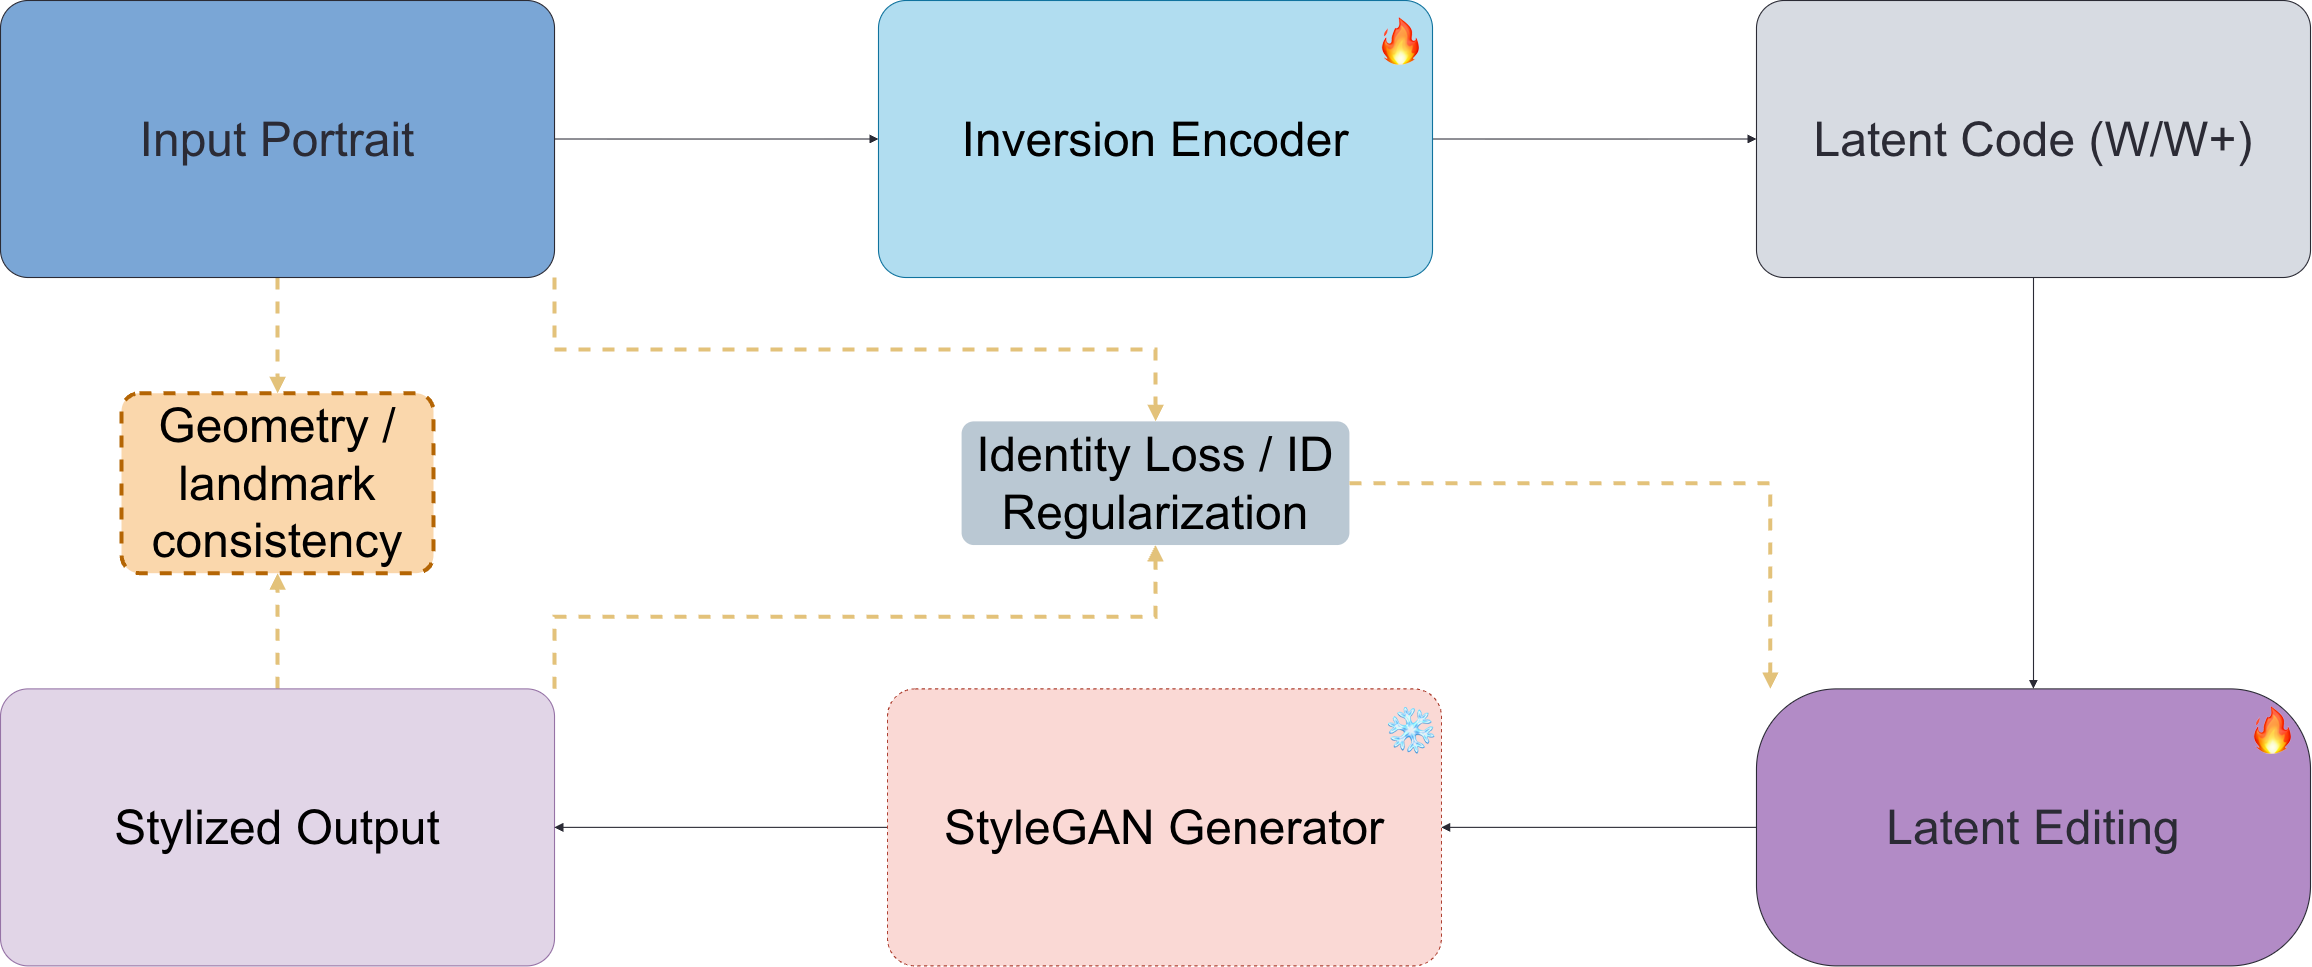
\includegraphics[width=0.98\textwidth]{images/pipeline.png}
  \caption{StyleGAN inversion and latent editing workflow for portrait stylization. The diagram highlights the main forward path and auxiliary identity/geometry regularization branches.}
  \label{fig:stylegan_pipeline}
\end{figure*}

\textbf{Advantages:} GANs are well-known for \textit{inference efficiency} (often interactive) and strong \textit{visual fidelity}. Because the generator is inherently constrained by the human face manifold (e.g., FFHQ), it naturally preserves identity structure and produces ultra-high-resolution, photorealistic details without catastrophic geometric collapse.

\textbf{Limitations:} A central limitation of GAN-based systems is \textit{domain lock-in}. They strictly require face images to be meticulously cropped and aligned. Furthermore, their generative capacity is heavily bounded by the training distribution; they struggle to generalize to open-vocabulary, out-of-domain artistic concepts (e.g., "cyberpunk robot face") without undergoing computationally expensive domain-specific fine-tuning.

% ==========================================
% 3.3 Diffusion-Based Methods
% ==========================================
\subsection{Diffusion Models: Open-Domain Texture Synthesis}
\label{sec:methodology:diffusion}

\textbf{Core Mechanism:} Diffusion models formulate image generation as a reverse Markov chain, iteratively denoising a Gaussian distribution conditioned on textual or visual prompts \cite{ho2020denoising}. For portrait stylization, the mechanism relies on manipulating the UNet's attention layers. Textual or visual style cues are injected into \textit{Cross-Attention} layers, while structural identity is maintained by swapping the Key ($K$) and Value ($V$) matrices in \textit{Self-Attention} layers with those of the source image. Recent advances freeze the backbone and train lightweight \textit{Adapters} to decouple identity embeddings (e.g., via ArcFace) from style conditionings.

\textbf{Representative Methods (Coverage: $\sim$45 papers):} This is currently the most heavily researched paradigm. This count includes directly discussed methods and cited baselines within the referenced works.
1) \textit{Fine-tuning methods:} DreamBooth~\cite{ruiz2023dreambooth} and Textual Inversion~\cite{gal2022image} paved the way for subject-driven generation, with ProSpect \cite{zhang2023prospectps}, StyleDrop \cite{sohn2023styledrop}, ZipLoRA \cite{shah2023ziplora}, and DiffStyler \cite{huang2024diffstyler} extending controllable style personalization under low-rank or dual-path adaptation.
2) \textit{Training-free methods:} InstantStyle \cite{wang2025instantstyleplus}, StyleAligned \cite{hertz2023styleai}, Style Injection \cite{chung2023styleii}, MasaCtrl \cite{cao2023masactrl}, ZeCon \cite{yang2023zecon}, Visual Style Prompting \cite{jeong2024visualsp}, FreeStyle \cite{he2024freestylefl}, Zero-Shot CLIP \cite{yang2023zeroshotcl}, and DiffuseIT \cite{kwon2022diffuseit} achieved zero-shot transfer via attention-control and feature-guidance mechanisms. To accelerate the process, ZePo \cite{liu2024zepozp} and DEADiff \cite{qi2024deadiff} introduced efficient stylization paths without full model retraining.
3) \textit{Adapters:} InstantID \cite{wang2024instantid}, StyleBooth \cite{han2024styleboothis}, MagicFace \cite{wang2024magicfacetu}, Visual Concept Translator \cite{cheng2023visual}, StyleTokenizer \cite{li2024styletokenizerdi}, and CreativeSynth \cite{huang2024creativesynthcf} utilized lightweight conditioning modules to bind identity, style tokens, and cross-art attention signals.

4) \textit{Inversion and editing:} DiffusionCLIP \cite{kim2022diffusionclip} remains a representative text-guided inversion/editing baseline in portrait-centric diffusion pipelines. Inversion-based style transfer further extends diffusion to explicit content--style decomposition \cite{zhang2022inversionbasedst}.

Beyond the adapters above, a wave of 2024--2025 works targets identity-preserving and tuning-free stylization on diffusion backbones. PhotoMaker~\cite{li2024photomaker} stacks ID embeddings for efficient personalized portrait generation, while PULID~\cite{guo2024pulid} and ConsistentID~\cite{huang2024consistentid} improve ID fidelity through contrastive alignment and multimodal fine-grained identity control, respectively. For pure style transfer, StyleShot~\cite{gao2024styleshot} introduces a style-aware encoder with a decoupling strategy to mimic arbitrary reference styles without test-time tuning. Together these works show a clear shift from full fine-tuning toward lightweight, identity-aware, and test-free diffusion stylization.

Closely related, rectified-flow and flow-matching editors (e.g., FlowEdit, DVRF, FlowAlign, introduced in Section~\ref{sec:foundations:flow}) reformulate stylization as a deterministic optimal-transport ODE, providing inversion-free editing with stronger structure retention than stochastic diffusion sampling \cite{flowedit2025,dvrf2025,flowalign2025}.

\textbf{Advantages:} Diffusion models offer \textit{unprecedented semantic diversity} and open-vocabulary control. Unlike GANs, they are not constrained by facial alignment and can seamlessly stylize the portrait alongside complex backgrounds, lighting, and out-of-domain aesthetic concepts.

\textbf{Limitations:} The trade-off is \textit{computational latency} and \textit{content leakage}. Iterative denoising (typically 30--50 steps) prohibits real-time video deployment. Furthermore, without strict spatial constraints, the model frequently suffers from "content leakage"—where semantic elements from the style reference (e.g., a flower, a hat) erroneously bleed onto the subject's face.

% ==========================================
% 3.4 AR and Transformer Models
% ==========================================
\subsection{Autoregressive Models: Bridging Discrete Tokens and Global Structure}
\label{sec:methodology:ar}

Recent empirical results highlight the competitiveness of this paradigm. For example, EditAR \cite{mu2025editar} achieves a comprehensive CLIP score of 75.13 and an edited region CLIP score of 39.43 on the PIE-Bench dataset, significantly outperforming many traditional inversion-based baselines in unified conditional generation.

\textbf{Core Mechanism \& Theoretical Basis:} Unlike continuous latent diffusion or GANs, Autoregressive (AR) and Transformer-based models treat image generation as a sequential discrete prediction task. The foundational theory relies on Vector Quantized Variational Autoencoders (VQ-VAE), which compress high-dimensional portraits into a grid of discrete visual tokens \cite{esser2021vqgan}. Stylization is subsequently formulated as predicting the probability distribution of the next token given a sequence of prior tokens and a condition (e.g., text or style reference). By leveraging the global receptive field of self-attention mechanisms, AR models theoretically avoid the local inductive biases of CNNs, capturing long-range structural dependencies.

\textbf{Representative Methods (Coverage: $\sim$10 papers):} The paradigm was popularized by VQGAN \cite{esser2021vqgan}, which introduced adversarial losses to the quantization process for higher fidelity. To overcome the slow unidirectional decoding of standard AR models, MaskGIT \cite{chang2022maskgit} proposed bi-directional masked image modeling, processing tokens in parallel. Recently, the Visual Autoregressive (VAR) framework \cite{tian2024var} shifted the modeling from "next-token" to "next-scale" prediction, while Infinity \cite{han2024infinity} demonstrated large-scale bitwise AR synthesis at higher resolution. This theoretical leap has been adapted by EditAR \cite{mu2025editar}, enabling unified conditional generation and structural stylization without the heavy iterative denoising required by diffusion models.

\textbf{Advantages:} The primary strength of AR models lies in their \textit{structural coherence}. Because transformers model global attention, they excel in handling extreme geometric abstractions (e.g., Picasso-style cubism or exaggerated manga) where local convolution windows typically induce structural drift or facial collapse.

\textbf{Limitations:} The reliance on a discrete codebook fundamentally restricts the preservation of high-frequency identity details (e.g., fine skin pores or individual hair strands), leading to \textit{quantization artifacts}. Furthermore, scaling these models demands enormous computational resources and massive datasets to prevent the sequence predictions from degenerating during complex style adaptations.

\begin{table*}[t]
\centering
\caption{Capability matrix of representative PST methods. Qualitative symbols: $\bigstar$ = strong/fast; $\blacktriangle$ = moderate; $\bullet$ = weak/slow. Numeric values are indicative under each method's original evaluation protocol.}
\label{tab:comparison_matrix}
\small
\setlength{\tabcolsep}{3.5pt}
\begin{tabular}{lcccp{1.8cm}cl}
\toprule
\textbf{Method} & \textbf{Paradigm} & \textbf{Identity} & \textbf{Setup} & \textbf{Speed} & \textbf{Limitation} \\
\midrule
Gatys et al.~\cite{gatys2015ana} & NST & Gram matrix & Opt., style img & $\bullet$~min & Structural drift \\
AdaIN~\cite{huang2017arbitraryst} & NST & AdaIN stats & FF, style set & $\bigstar$~$<$1s & Washed-out texture \\
Deep Photo~\cite{luan2017deepps} & NST & Semantic corresp. & Opt., style img & $\bullet$~min & Semantic misalign. \\
\midrule
DualStyleGAN~\cite{yang2022dualstylegan} & GAN & Intrinsic/extrinsic path & FF, StyleGAN & $\bigstar$~$<$1s & Domain lock-in \\
pSp/e4e~\cite{richardson2021encoding} & GAN & Encoder $W^+$ inv. & FF, enc. trn. & $\blacktriangle$~sec & Inv. quality trade-off \\
AgileGAN~\cite{song2021agilegan} & GAN & Hier. VAE $W^+$ inv. & FF, few-shot & $\bigstar$~130ms & Geometric collapse \\
VToonify~\cite{yang2022vtoonify} & GAN & Multiscale feat.+StyleGAN & FF, StyleGAN ft. & $\bigstar$~real-time & Domain bound \\
\midrule
InstantID~\cite{wang2024instantid} & Diff. & ArcFace cross-attn. & FF, zero-shot & $\blacktriangle$~sec & Content leakage \\
IP-Adapter~\cite{ye2023ipadapter} & Diff. & Decoupled cross-attn. & FF, adapt. trn. & $\blacktriangle$~sec & Style bleeding \\
DreamBooth~\cite{ruiz2023dreambooth} & Diff. & Subject token tuning & FT, few-shot & $\bullet$~min & Catastr. overfit \\
StyleMaster~\cite{ye2024stylemastersy} & Diff. & Motion adapt.+global proj. & FF, 10K pairs & $\blacktriangle$~0.6s & Flicker \\
FlowEdit/DVRF~\cite{flowedit2025,dvrf2025} & Diff. & Rectified-flow ODE & FF, inversion-free & $\bigstar$~sec & Trajectory tuning \\
\midrule
EditAR~\cite{mu2025editar} & AR & Feat. distill.+tokens & FF, large-scale & $\bigstar$~$<$1s & Quantiz. artifacts \\
VAR~\cite{tian2024var} & AR & Next-scale predict. & FF, large-scale & $\bigstar$~0.8s & Codebook collapse \\
MaskGIT~\cite{chang2022maskgit} & AR & Bidir. masked modeling & FF, large-scale & $\bigstar$~$<$1s & Resolution limit \\
\bottomrule
\end{tabular}
\setlength{\tabcolsep}{6pt}
\end{table*}

\textbf{Takeaway:} Across these four families (summarized in Table~\ref{tab:comparison_matrix}), portrait stylization methods consistently trade off geometric faithfulness, texture controllability, and computational efficiency, with no single paradigm dominating all constraints simultaneously. In practice, modern systems increasingly adopt hybrid pipelines (e.g., diffusion backbones with adapter/inversion controls) to recover identity while preserving open-domain stylization capacity. This taxonomy therefore serves as the technical basis for the task-level analysis and benchmark interpretation in the following sections.

\section{Advanced Stylization Tasks and Applications}
\label{sec:advanced}
Beyond the core paradigms above, portrait stylization extends along three dimensions of increasing complexity: from global 2D editing toward fine-grained local control, from static images to temporally coherent video, and from 2D to 3D-aware multiview generation. This section surveys these advanced tasks, organized by the spatial, temporal, and geometric dimensions they address.

\subsection{Video Portrait Stylization (Temporal Consistency)}
\label{sec:advanced:video}
Video portrait stylization extends static style transfer to temporal sequences, where professional-grade results require both temporal coherence and identity stability \cite{ruder2018artistic,ye2024stylemastersy,huang2023styleavideoad,yang2023rerender,liu2023portraitdt,yang2024fresco}. While per-frame stylization is straightforward, the central technical challenge is to prevent high-frequency temporal variance from producing perceptually disruptive artifacts.

The primary hurdle is \emph{flickering}: inconsistent stylization across consecutive frames that breaks the viewer's suspension of disbelief \cite{ye2024stylemastersy}. Temporal consistency is commonly formalized through optical-flow-based warping losses. Given consecutive frames $I_t, I_{t-1}$ and estimated optical flow $F_{t\to t-1}$, a warping loss encourages the stylized frames to be consistent under motion:
\begin{equation}
\mathcal{L}_{warp} = \sum_{t} \bigl\lVert \phi(I_t) - \mathcal{W}\bigl(\phi(I_{t-1}), F_{t\to t-1}\bigr) \bigr\rVert_1,
\end{equation}
where $\phi(\cdot)$ denotes a feature extractor (e.g., VGG layers) and $\mathcal{W}$ is the backward warping operation. A temporal perceptual loss further penalizes feature deviations across warped pairs:
\begin{equation}
\mathcal{L}_{temp} = \sum_{t,l} \bigl\lVert \Phi_l(I_t) - \Phi_l\bigl(\mathcal{W}(I_{t-1}, F_{t\to t-1})\bigr) \bigr\rVert_2^2,
\end{equation}
with $\Phi_l$ the activations at layer $l$ of a pretrained network. These formulations, adopted by Ruder et al. \cite{ruder2018artistic} and refined in later portrait-specific pipelines, provide a principled basis for enforcing cross-frame coherence beyond simple per-frame stylization.

Furthermore, ReRender-A-Video \cite{yang2023rerender} proposes a zero-shot, text-guided video translation framework that enforces hierarchical cross-frame constraints to maintain global style coherence without requiring expensive per-video fine-tuning. Achieving temporal consistency is a non-trivial extension of both GAN and diffusion paradigms, since the model must accommodate motion while preserving identity-critical facial cues.

\subsubsection{StyleMaster: Decoupling Motion and Style}
\label{sec:advanced:video:stylemaster}
StyleMaster addresses temporal dynamics via architectural decoupling that separates stylistic features from structural motion \cite{ye2024stylemastersy}. It introduces a dedicated motion adapter (an auxiliary U-Net-like network) to model temporal cues without contaminating the main stylization manifold. To reduce content leakage and preserve structure, the framework further employs a global projection mechanism together with regularization (e.g., variational Laplacian regularization) that smooths transitions between source and target domains. Temporal stability is evaluated using consistency-oriented metrics (e.g., UMT/CSD-like scores) that quantify the smoothness of stylization over time.

\subsubsection{Conditional Guidance in Style-A-Video}
\label{sec:advanced:video:styleavideo}
In contrast to architectural modification, conditional-guidance methods (e.g., Style-A-Video) combine input frames, text prompts, and attention maps to steer stylization \cite{huang2023styleavideoad}. Attention maps provide spatial control, enabling styles to be applied along semantic boundaries rather than by global latent manipulation.

\subsubsection{Consistency Baselines}
\label{sec:advanced:video:baselines}
Methods such as VToonify are commonly used as baselines for video consistency, emphasizing cross-frame correspondence to reduce flicker \cite{yang2022vtoonify}. However, achieving fine-grained control over facial attributes typically requires moving beyond global video stylization toward localized editing.

For transparency, currently available reports in this survey's source set do not provide a unified CelebV-HQ benchmark table with FID/CLIP-S/ID-Sim simultaneously reported for StyleMaster, VToonify-D, and ReRender-A-Video under one protocol. We therefore avoid constructing a pseudo-comparable numeric ranking in this subsection.

Complementary to stylization-specific pipelines, general portrait video generation has advanced rapidly in 2024--2025. AnimateDiff~\cite{guo2024animatediff} animates personalized text-to-image diffusion models without task-specific tuning, while MagicAnimate~\cite{xu2024magicanimate} and AnimateAnyone~\cite{hu2024animateanyone} focus on temporally consistent human-image and character animation driven by pose signals. LivePortrait~\cite{guo2024liveportrait} further enables efficient portrait animation with stitching and retargeting control for expressive facial motion. These methods supply the motion and identity priors that downstream portrait stylization can build upon.

\subsection{Local Editing and Makeup Transfer (Fine-grained Control)}
\label{sec:advanced:local}
Local editing shifts the goal from global stylization to region-specific manipulation (e.g., lips or eyes) while preserving skin texture and global identity. This introduces a ``precision paradox'': commercial scenarios such as virtual try-on demand near-perfect identity preservation, yet require high-frequency local texture changes without introducing artifacts in non-target regions \cite{yan2023facestudiopy,liu2023portraitdt,ambiel2023portraitsa}. Cross-domain cartoon/manga stylization (e.g., photo-to-manga) further exemplifies the precision--fidelity trade-off under extreme stylization \cite{su2021mangagan}.

\subsubsection{Stable-Makeup: Prompt-guided Local Control}
\label{sec:advanced:local:stablemakeup}
Stable-Makeup \cite{zhang2024stablemakeup} explicitly separates identity prompts from instruction prompts. These diffusion-based makeup systems combine CLIP-derived detail features with ControlNet-style structural constraints (a paradigm also shared by FreeUV \cite{yang2025freeuv}) to preserve geometry.

\subsubsection{Baselines and Data Synthesis}
\label{sec:advanced:local:baselines}
Classic GAN-based baselines include BeautyGAN \cite{li2018beautygan}, PSGAN \cite{jiang2020psgan}, and LADN \cite{gu2019ladn}, which emphasize robust spatial alignment and local-region transfer under pose/expression variation. EleGANt further improves local editability through style-to-source alignment and shifted-window attention, and reports reconstruction-oriented metrics on MT-Eval and Makeup-Wild \cite{yang2022elegant}. More recent editing/synthesis pipelines (e.g., prompt-guided editors) can also generate pseudo-paired data or guidance signals that encourage high-frequency cosmetic detail without corrupting non-target facial regions. At the intersection of local editing and global compositing, Barbershop~\cite{zhu2021barbershop} performs GAN-based image compositing using segmentation masks to transplant local attributes (e.g., hair) between portraits while preserving surrounding identity, illustrating the precision--fidelity trade-off in localized portrait manipulation.

\subsection{3D-Aware Portrait Stylization}
\label{sec:advanced:3d}
Current methodologies for 3D-aware stylization are rapidly transitioning from Neural Radiance Fields (NeRF) to 3D Gaussian Splatting (3DGS) due to the latter's explicit geometric representation and real-time rendering capabilities. Recent pioneering works, such as 3DToonify \cite{threedtoonify2024} and StyleSplat \cite{jain2024stylesplat}, have demonstrated high-fidelity stylized avatar creation by coupling 3DGS with diffusion priors.

To address multi-view inconsistency and rendering latency, a series of concurrent works in 2024--2025 have further extended these frameworks. While NeRF-based methods prioritize continuous volumetric quality, emerging 3DGS adaptations specifically target sub-second interactive rendering (as self-reported in recent concurrent literature, though standard cross-platform benchmarks remain to be independently verified) and dynamic audio-driven expressions. Despite these rapid advances, decoupling non-rigid topological deformations (e.g., exaggerated anime eyes) from static appearance fields without causing catastrophic geometric collapse remains a critical open challenge. The 2024--2025 3DGS wave also brings specialized portrait components. 3DGS-Avatar~\cite{qian20243dgsavatar} models animatable avatars via deformable 3D Gaussian splatting with explicit skeletal control, while GaussianHair~\cite{luo2024gaussianhair} reconstructs and renders hair using light-aware Gaussians for photorealistic strand-level detail. Such components extend stylized avatars from holistic appearance toward disentangled, animatable, and high-frequency geometry. Earlier NeRF-based stylization laid the groundwork: NeRF-Art~\cite{wang2022nerf} performs text-driven 3D scene stylization, while StylizedNeRF~\cite{huang2022stylizednerf} extends radiance-field stylization to portraits.

\subsubsection{Key Technical Challenges}
The primary obstacle lies in disentangling rigid topology from stylistic textures. Methods such as those by Feng and Singhal \cite{feng20233dfs} utilize hybrid NeRF and mesh rasterization to address this. Current 3DGS implementations must balance texture and aesthetic guidance while ensuring the underlying canonical face mesh does not collapse during extreme artistic stylization.
\label{sec:advanced:3d:rigging}
3D-aware control mechanisms leverage parametric facial models and semantic directions (pose, expression, age) to preserve structural controllability during stylization. Such rigging-style controls provide stable geometry priors that help maintain identity under multi-view rendering.

\subsubsection{Texture and Aesthetic Guidance}
\label{sec:advanced:3d:guidance}
Depth-heavy aesthetics can be encouraged using 3D-oriented prompts (e.g., ``3D render'' or ``clay'' styles) and lighting-aware objectives, improving volumetric plausibility of highlights and shadows. Combining multi-view constraints with semantic guidance remains a key direction toward immersive, consistent avatars \cite{jain2024stylesplat}.

\subsection{Summary}
\label{sec:advanced:summary}
For 3D-aware tasks, while static NeRFs provide high-fidelity novel views, dynamic 3DGS methods trade some geometric rigidity for sub-second rendering and real-time animatability. For a structured comparison of open challenges across these advanced task domains, see Table \ref{tab:research_roadmap} in Section \ref{sec:discussion}. Overall, advanced portrait tasks push PST beyond global 2D stylization toward temporal coherence, fine-grained local control, and multi-view consistency. These settings typically require specialized auxiliary networks, stronger regularization, and structure-aware controls to maintain identity under significantly more demanding constraints \cite{ye2024stylemastersy,jain2024stylesplat}.

\section{Evaluation Metrics and The Benchmark Protocol}
\label{sec:evaluation}

In portrait style transfer, evaluation must account for a delicate duality: the biometric sensitivity of human faces and the deliberate structural deviations introduced by abstract artistic intent. Standard reconstruction-oriented metrics frequently fail to capture these nuances, often penalizing highly creative stylizations as "geometric distortions."

Before presenting the Golden Protocol configuration, we survey which metrics the surveyed PST methods actually report (Table~\ref{tab:metric_usage}). The pattern reveals two gaps: first, ArtFID---arguably the most holistic single metric---is adopted by fewer than 10\% of methods, most published after 2023; second, fewer than 20\% of papers report user studies, and those that do vary widely in sample size and statistical rigor. This fragmentation motivates the standardized protocol below.

\begin{table*}[t]
\centering
\caption{Metric reporting frequency across paradigms. "Common" = $\ge$50\% of methods, "Occasional" = 10--50\%, "Rare" = $<$10\%. N/A* denotes a metric unavailable at the paradigm's inception (e.g., LPIPS \cite{zhang2018lpips} was proposed in 2018, after classic NST \cite{gatys2015ana,gatys2016image}), and is only applied retrospectively in later works.}
\label{tab:metric_usage}
\small
\begin{tabular}{lcccc}
\toprule
\textbf{Metric} & \textbf{NST} & \textbf{GAN} & \textbf{Diffusion} & \textbf{AR} \\
\midrule
FID / KID        & Rare & Common & Common & Rare \\
LPIPS            & N/A*   & Occasional & Occasional & Rare \\
ID Score (ArcFace) & Rare & Common & Common & Occasional \\
CLIP Score       & Rare & Rare & Common & Common \\
ArtFID           & Rare & Rare & Occasional & Rare \\
User Study       & Occasional & Common & Occasional & Rare \\
\bottomrule
\end{tabular}
\end{table*}

To address the inconsistencies highlighted in prior works and improve cross-paper reproducibility, we formalize a comprehensive benchmark framework, termed the \textbf{"Golden Protocol"} (a \textit{proposed} guideline; it is \underline{not} empirically executed within this survey, which only surveys existing reports). This protocol recommends a multi-pillar approach encompassing standardized experimental configurations, distribution-aware quantitative metrics, and rigorous human-centric qualitative studies.

% ==========================================
% 5.1 Standardized Configuration & Reproducibility
% ==========================================
\subsection{The Golden Protocol: A Proposed Benchmark Guideline}
\label{sec:evaluation:configuration}

A persistent flaw in current literature is the "cherry-picking" of style-content pairs. To ensure a fair and reproducible evaluation, the Golden Protocol recommends that researchers report the following standardized configurations:

\begin{itemize}
\item \textbf{Dataset Standardization:} Evaluations should be conducted on universally recognized test splits. We recommend sampling 1,000 to 5,000 paired combinations using high-quality content datasets (e.g., FFHQ or CelebA-HQ) and specific style domains (e.g., WikiArt for textures, Danbooru for anime, or AAHQ for artistic portraits). For prompt-based models, standard prompt suites from OmniStyle-1M (see Section~\ref{sec:datasets:omnistyle}) should be utilized to test long-tail style vocabularies.
\item \textbf{Sampling \& Hyperparameters:} For diffusion-based models, authors should report the inference settings: the choice of sampler (e.g., DDIM), the exact number of denoising steps (typically 30--50 steps for training-free methods), and the Classifier-Free Guidance (CFG) scale.
\item \textbf{Reporting Format:} All quantitative results should be aggregated over fixed random seeds (e.g., 3-5 seeds per prompt/image) and reported in a strict \textit{Mean $\pm$ Standard Deviation} format. For deterministic models (e.g., GAN-based), seed variation applies to inversion optimization; report mean $\pm$ std over 3-5 inversion runs.
\end{itemize}

% ==========================================
% 5.2 Multi-Pillar Quantitative Metrics
% ==========================================
\subsection{Multi-Pillar Quantitative Benchmarking}
\label{sec:evaluation:quantitative}

Following the configurations above, the generated outputs should be assessed along three distinct axes to reflect the Portrait Editing Trilemma:

\textbf{1) Identity Integrity (ID Score):} Identity preservation is measured by computing the cosine similarity between the deep facial embeddings of the source and stylized images using pre-trained recognition models (e.g., ArcFace \cite{deng2019arcface} or CurricularFace), and this protocol is widely adopted by portrait-specific baselines such as StyleFace \cite{sain2023styleface}.
\textit{Critical Caveat:} It is crucial to acknowledge that ID networks are trained on photorealistic domains. When applied to abstract or exaggerated styles (e.g., Cubism or Caricatures), the ID Score naturally degrades despite human recognizable likeness. Thus, ID Scores should only be compared strictly within the same target style domain.

\textbf{2) Holistic Style-Content Trade-off (ArtFID):} Relying solely on Style Loss often leads to texture overfitting, while raw FID \cite{heusel2017ttur} ignores spatial content. We recommend \textbf{ArtFID} \cite{wright2022artfidqe} as the primary distributional metric. ArtFID mathematically balances content drift and style matching by combining LPIPS \cite{zhang2018lpips} and FID: $\text{ArtFID} = (1 + \text{LPIPS}) \cdot (1 + \text{FID})$. A lower ArtFID indicates a highly stylized image that structurally respects the source content.

\emph{Limitations:} ArtFID inherits the biases of its components. LPIPS, pretrained on photorealistic image pairs, penalizes non-photorealistic distortions intrinsic to artistic styles (e.g., visible brushstrokes or line distortions in caricatures). FID, computed on Inception features trained on ImageNet, is sensitive to texture statistics and may mis-rank methods that produce stylistically diverse outputs within the same domain \cite{wright2022artfidqe}. Consequently, ArtFID should be interpreted as a holistic ranking tool rather than an absolute quality measure; cross-paradigm comparisons (e.g., GAN vs.\ diffusion) are meaningful only when evaluated on the same test set and style domain.

\textbf{3) Cross-Modal Semantic Alignment (CLIP Score):} For open-domain text-driven methods, CLIP-T measures the cosine similarity between the stylized image and the driving textual prompt in the CLIP embedding space \cite{radford2021learningtv}. Similarly, CLIP-I is used to measure visual stylistic alignment between the output and a reference style image without requiring paired ground truths.

% ==========================================
% 5.3 Human Studies and LMM Proxies
% ==========================================
\subsection{Qualitative Evaluation: Human Studies and LMM Proxies}
\label{sec:evaluation:qualitative}

Because stylization quality is ultimately determined by human perception, objective metrics must be anchored by rigorous subjective evaluation.

\textbf{Human A/B Testing Protocol:} We standardize the user study methodology to a Two-Alternative Forced Choice (2AFC) or a Mean Opinion Score (MOS) framework \cite{streijl2016mean}. Evaluators must score outputs on a 5-point Likert scale across three isolated criteria: \textit{(i) Identity Preservation}, \textit{(ii) Style Faithfulness}, and \textit{(iii) Overall Aesthetic Preference}.

\emph{Methodological considerations.} Surveying current user studies in PST reveals wide variability: sample sizes range from 10 to 100+ raters per condition, and fewer than half report inter-rater reliability (e.g., Fleiss' Kappa or Krippendorff's Alpha) \cite{selim2016portrait,yi2019apdrawinggan}. Best practices from perceptual quality assessment recommend at least 20--30 raters per condition for MOS and 15+ pairwise comparisons per pair for 2AFC designs to achieve 80\% statistical power at $\alpha = 0.05$ \cite{streijl2016mean}. To further reduce demographic bias in aesthetic judgments, rater pools should include diverse age, gender, and cultural backgrounds.

While current literature coverage of ArtFID remains limited, we strongly call for its adoption as a standard metric in future PST benchmarks to unify aesthetic evaluation.

\textbf{Large Multimodal Models (LMMs) as Evaluators:} Driven by the high cost of human crowdsourcing, recent pipelines incorporate advanced LMMs (e.g., GPT-4o \cite{hurst2024gpt4o}) as scalable proxies for qualitative scoring. Under the Golden Protocol, when using LMMs, the evaluation prompt should be explicitly structured to mimic human cognitive processes via Chain-of-Thought (CoT) reasoning. The prompt should explicitly instruct the LMM to disentangle "biometric preservation" from "stylistic abstraction".

\emph{Current limitations and calibration.} Despite their promise, LMM-based evaluation introduces systematic biases. Recent benchmarks show LMMs exhibit position bias, authority bias, and sensitivity to superficial visual features (e.g., color saturation and contrast), while under-detecting high-frequency artifacts such as texture swimming \cite{chen2024mllmjudge}. Moreover, LMM judgments lack the perceptual grounding of human vision; they are trained on caption--image alignment rather than aesthetic preference. Calibration strategies---including multi-prompt aggregation, temperature averaging over repeated trials, and human-anchored normalization---can reduce but not eliminate these distortions. We therefore recommend LMM scores as a rapid screening tool rather than a replacement for formal user studies.

\paragraph{Visual Artifact Analysis and Failure Modes.}
Qualitative evaluation should further categorize failure modes from existing methods: (i) \textit{content leakage}, where unintended semantic elements from a style reference (e.g., hats, signatures, background objects) bleed into the portrait via entangled cross-attention, and (ii) \textit{identity distortion}, where geometric changes to facial components break recognizability. A recurring pitfall is high-strength stylization: pushing style strength beyond a paradigm-specific threshold can cause identity collapse into a generic face in the target domain. Reporting such failure cases alongside aggregate metrics is essential for a complete evaluation picture.

\section{Datasets, Privacy, and Ethical Benchmarks}
\label{sec:datasets}

The evolution of portrait style transfer has been fundamentally reshaped by the transition from classical optimization to data-driven generative modeling. In this modern paradigm, datasets are no longer passive evaluation references; they act as the primary generative engine that defines the bounds of the learned latent manifolds. However, as the field matures, the focus has shifted from merely scraping massive uncurated image collections to constructing high-fidelity, legally compliant, and strictly paired generative benchmarks.

% ==========================================
% 6.1 Content & Style Datasets (with License & Privacy)
% ==========================================
\subsection{Content and Style Datasets: The Privacy Shift}
\label{sec:datasets:content_style}

\textbf{Content Datasets and Privacy Compliance.} In common research practice, dataset deployment must navigate strict licensing constraints rather than relying solely on technical availability. For instance, FFHQ provides specific opt-out mechanisms for privacy compliance\footnote{See maintainer documentation: \url{https://github.com/NVlabs/ffhq-dataset}}, while CelebA-HQ and Danbooru carry varying degrees of commercial restriction and copyright risks\footnote{Refer to community compliance guidelines regarding scraped datasets for non-commercial research.}. To mitigate these legal risks, recent methodologies are pivoting towards large-scale synthetic datasets.

\textbf{Style Repositories.} To define the artistic target domain, researchers predominantly utilize WikiArt \cite{wikiart} (250,000+ general artworks) for global brushstroke modeling, and Danbooru \cite{danbooru2021} for tag-based controllable anime stylization. For human-centric artistic portraits, AAHQ \cite{liu2021blendgan} (25,000+ curated artistic faces) serves as a robust benchmark to prevent models from collapsing into a generic "average" artistic style.

% ==========================================
% 6.2 Large-Scale Synthetic Data: The OmniStyle-1M Paradigm
% ==========================================
\subsection{Large-Scale Synthetic Triplets: The OmniStyle-1M Paradigm}
\label{sec:datasets:omnistyle}

Historically, the advancement of supervised style transfer and instruction-guided editing was severely hindered by the scarcity of "ground-truth" stylization pairings (i.e., exact photo-to-art counterparts). Open-vocabulary models frequently fail on long-tail styles because they lack explicit structural alignment in their training distribution.

To bridge this critical gap, Wang et al. \cite{wang2025omnistyle} recently introduced \textbf{OmniStyle-1M}, a massive dataset comprising over one million highly curated triplets: (1) a content image, (2) a style reference, and (3) the resulting stylized output, spanning 1,000 fine-grained style categories.

\textbf{Data Generation and OmniFilter:} The construction of OmniStyle-1M represents a paradigm shift in automated dataset curation. Content images across 20 categories are initially synthesized using the FLUX model combined with ChatGPT-generated prompts. To ensure diverse style representations, six strong transfer models are employed to generate candidate stylized results. Crucially, to eliminate structural drift and style degradation, the authors proposed \textbf{OmniFilter}, an automated evaluation pipeline utilizing Large Multimodal Models (LMMs, such as InternVL). OmniFilter strictly scores each generated triplet across three explicit axes: \textit{Content Preservation} (semantic and structural integrity), \textit{Style Consistency}, and \textit{Aesthetic Appeal}. Only triplets passing this rigorous filtering are retained. Training on this strictly aligned, explicitly filtered triplet data enables current Diffusion Transformers (DiT) to achieve highly predictable and artifact-free zero-shot stylizations \cite{wang2025omnistyle}. Since content images in OmniStyle-1M are AI-synthesized, downstream models may inherit generative biases from FLUX; complementary evaluation on real-face datasets (e.g., FFHQ) is strongly recommended.

% ==========================================
% 6.3 Dataset Selection Guide
% ==========================================
\subsection{Dataset Selection Guide for Practitioners}
\label{sec:datasets:guide}

Selecting the appropriate dataset is the most critical determinant of a model's operational success. Based on our comprehensive review, we provide the following selection guide for researchers navigating specific sub-tasks:

\begin{itemize}
\item \textbf{Global Texture and Arbitrary Stylization:} For general-purpose texture synthesis without strict semantic boundaries, training on \textbf{WikiArt} paired with \textbf{FFHQ} remains the foundational baseline.
\item \textbf{Local Editing and Makeup Transfer:} Tasks requiring precise spatial disentanglement (e.g., eye-makeup or lip-color transfer) should utilize \textbf{CelebAMask-HQ} for its dense parsing maps, alongside the paired synthetic \textbf{CPM} dataset \cite{nguyen2021lipstick} to learn supervised cosmetic attributes.
\item \textbf{Video Temporal Consistency:} For video portrait stylization aiming to reduce frame flickering, \textbf{CelebV-HQ} \cite{celebvhq} (containing over 35,000 high-quality video clips) is the mandatory benchmark for evaluating optical flow and cross-frame attention mechanisms.
\item \textbf{Open-Vocabulary and Instruction Editing:} For modern text-driven or multi-modal diffusion adapters handling long-tail prompts (e.g., "cyberpunk watercolor"), pre-training on the million-level triplets of \textbf{OmniStyle-1M} \cite{wang2025omnistyle} provides the necessary semantic alignment that raw uncurated datasets lack. (Its content images are AI-synthesized; we refer to Section~\ref{sec:datasets:omnistyle} for the bias-mitigation note and the recommendation to complement with real-face datasets such as FFHQ.)
\end{itemize}

\begin{table*}[t]
\centering
\caption{Summary of Key Datasets in Portrait Style Transfer, including License and Compliance Status.}
\label{tab:datasets_pst}
\begin{tabularx}{\textwidth}{lcrlp{2.8cm}p{3.2cm}}
\toprule
\textbf{Dataset} & \textbf{Year} & \textbf{Size} & \textbf{Type} & \textbf{License / Availability} & \textbf{Primary Utility} \\
\midrule
FFHQ \cite{karras2019style} & 2019 & 70k & Real Faces & CC BY-NC-SA 4.0 (Research) & High-res face prior for GAN inversion \\
CelebAMask-HQ \cite{lee2020} & 2020 & 30k & Real+Labels & Non-Commercial; redistrib.-sensitive & Semantic parsing for region-aware local editing \\
Danbooru \cite{danbooru2021} & 2021 & 4.9M & Anime Art & No explicit license; artwork copyright mixed (research/non-commercial) & Tag-based controllable anime stylization \\
WikiArt \cite{wikiart} & 2015 & 250k+ & Artworks & Public Domain (Mixed) & General artistic textures and brushstroke \\
AAHQ \cite{liu2021blendgan} & 2021 & 25k & Artistic Faces & CC BY-NC-SA 4.0 (Research) & Artistic portrait benchmark \\
OmniStyle-1M \cite{wang2025omnistyle} & 2025 & 1M & Synthetic Tr. & Open for Research & Text-image triplets for instruction editing \\
CelebV-HQ \cite{celebvhq} & 2022 & 35k clips & Real Video & Non-Commercial (Research) & Temporal consistency benchmarks for video \\
StyleGAN-Human \cite{stylegan-human} & 2022 & 40k+ & Synthetic F. & Open (Privacy-Compliant) & Diversity pretraining without real-face GDPR risk \\
\bottomrule
\end{tabularx}
\end{table*}

\section{Discussion and Open Challenges}
\label{sec:discussion}
\subsection{The Portrait Editing Trilemma in Practice}
\label{sec:discussion:triangle}
As established in Section~\ref{sec:intro:trilemma}, portrait stylization is governed by a multi-objective trade-off. In deployment, this tension appears as concrete operating points rather than a single optimum: systems with strong identity retention often limit stylization amplitude, while aggressively stylized outputs tend to reduce facial consistency or increase latency.
Recent systems explicitly analyze this structure when proposing single-step or adapter-based stylizers, revealing recurring constraints between realism, stylization strength, and runtime efficiency \cite{wang2025instantstyleplus,zhang2023prospectps}.

\subsection{Key Innovations under the Trilemma}
\label{sec:evaluation:innovations}
The current state of the art is shaped by the Trilemma---simultaneously achieving strong stylization intensity, high identity fidelity, and diverse outputs under practical compute budgets. Recent innovations increasingly rely on latent disentanglement and controlled feature modulation rather than pixel-level heuristics.

\subsubsection{Navigating the Style--Identity Trade-off}
\label{sec:evaluation:innovations:tradeoff}
A core idea is the statistical alignment hypothesis: It is widely hypothesized to encode structural/identity information \cite{huang2017arbitraryst}, though this mapping may not hold uniformly across all modern architectures. Systems that explicitly align or modulate these statistics provide a principled mechanism to balance identity and style.

\subsubsection{Computational Efficiency and Real-time Deployment}
\label{sec:evaluation:innovations:speed}
There is a clear trend toward training-free or forward-only generation for interactive applications. Techniques such as consistency-style distillation and fast samplers can substantially reduce inference latency under comparable settings, improving practical responsiveness on commodity hardware.

\subsubsection{Multimodal Control and Instruction Following}
\label{sec:evaluation:innovations:multimodal}
Modern systems increasingly support multimodal control (text + image + identity features). Decoupled conditioning mechanisms (e.g., separating identity and style streams in attention) reduce signal collapse and improve robustness under strong stylization, while parameter-efficient adapters enable diverse styles without catastrophic interference.

\subsection{Ethics, Regulation, and Deployment Constraints}
\label{sec:discussion:ethics_regulation}
The ethics discussion has shifted from generic ``responsible AI'' language to explicit regulatory compliance. Furthermore, the practical deployment of portrait stylization is increasingly governed by emerging global legal frameworks, such as the recently enacted Regulation (EU) 2024/1689 (EU AI Act) \cite{euaiact2024}. This imposes strict transparency obligations, requiring explicit watermarking or disclosure for AI-generated synthetic media to prevent misuse.

In parallel, GDPR treats identifiable facial embeddings as sensitive biometric data in many operational contexts. This creates concrete engineering requirements: data minimization, documented lawful basis, and executable deletion workflows aligned with right-to-erasure requests \cite{gdpr2016}. For subject-driven personalization models, this additionally implies lifecycle management of adapter checkpoints and cached identity embeddings, since preliminary security analyses indicate that these artifacts may potentially encode user-specific biometric traits, raising novel data privacy concerns regarding training data extraction and adversarial latent recovery \cite{carlini2023extracting, shamshad2023clip2protect}.

At the same time, the same technical advances that improve portrait stylization also lower the barrier for non-consensual synthetic media generation. This creates a direct co-evolution problem between stylization systems, deepfake detection pipelines, and provenance infrastructure: capability gains on the generation side can rapidly weaken detector robustness unless watermarking, traceability metadata, and post-deployment abuse monitoring are integrated by design.

Taken together, practical portrait stylization now requires a dual-stack design: (i) generation quality controls (identity/style/latency) and (ii) policy controls (consent, provenance, deletion, and auditability). Systems that optimize only visual metrics but omit compliance instrumentation face immediate deployment risk in regulated regions.

\section{Conclusion and Future Roadmap}
\label{sec:conclusion}

\subsection{Retrospective: Navigating the Trilemma}
\label{sec:conclusion:retrospective}
This decade-long survey (2015--2025) has chronicled the evolution of Portrait Style Transfer from heuristic texture matching to large-scale generative modeling. Returning to our analytical lens---the Portrait Editing Trilemma---we observe a clear historical shift in dominant paradigms. The ``Structure Masters'' (GANs, \cite{karras2019style}) dominated the mid-era by strictly bounding generation within the human face manifold, thereby solving the identity preservation problem but suffering from domain lock-in. The recent shift toward the ``Texture Masters'' (Diffusion Models, \cite{ho2020denoising,rombach_2022_cvpr}) broke these domain barriers, enabling open-vocabulary, zero-shot artistic stylization, yet re-introduced the challenges of identity loss and severe latency. We note, however, that this dichotomy is a historical generalization rather than a strict partition: many modern diffusion methods (e.g., IP-Adapter \cite{ye2023ipadapter}, InstantID \cite{wang2024instantid}) are explicitly designed for identity preservation, while certain GAN-based approaches offer broad stylistic diversity. The boundary continues to blur as hybrid designs emerge.

Currently, no single architecture perfectly satisfies the Trilemma. A broader emerging direction is multi-paradigm hybrid design, combining structured identity priors with open-vocabulary control to balance artistic intent and facial topology constraints.

\subsection{Open Challenges and Research Roadmap}
\label{sec:conclusion:roadmap}
Despite unprecedented visual fidelity, several fundamental bottlenecks remain unresolved. Based on our comprehensive review, we outline four critical open problems that define the immediate research roadmap for the field:

As summarized in Table~\ref{tab:research_roadmap}, these challenges can be mapped to concrete technical bottlenecks and actionable research trajectories.

\begin{table*}[t]
\centering
\caption{Research Roadmap for Portrait Style Transfer: Open Challenges and Proposed Trajectories.}
\label{tab:research_roadmap}
\begin{tabularx}{\textwidth}{l>{\raggedright\arraybackslash}X>{\raggedright\arraybackslash}X>{\raggedright\arraybackslash}X}
\toprule
\textbf{Open Challenge} & \textbf{Core Technical Bottleneck} & \textbf{Suggested Trajectory} & \textbf{Representative Works} \\
\midrule
\textbf{1. Video Temporal Consistency} & Independent frame sampling and cross-attention leakage cause high-frequency texture flickering. & Deterministic flow-guided attention; 4D continuous latent manifolds. & VToonify \cite{yang2022vtoonify}, StyleMaster \cite{ye2024stylemastersy}, ReRender-A-Video \cite{yang2023rerender}. \\
\textbf{2. 3D Geometric Stylization} & Rigid NeRF/3DGS priors collapse under large, non-rigid topological deformations. & Decoupling proxy from appearance fields; flow-matching regularizers. & 3DToonify \cite{threedtoonify2024}, FlowAlign \cite{flowalign2025}. \\
\textbf{3. Semantic "Content Leakage"} & Entangled CLIP spaces leak style-image semantics (e.g., hats) onto the target identity. & Explicit disentanglement of style/content tokens; cross-attention map isolation. & DEADiff \cite{qi2024deadiff}, InstantStyle \cite{wang2024instantstyle}. \\
\textbf{4. Sub-Second Inference} & Iterative denoising prohibits interactive, real-time avatar applications. & Single-step trajectory distillation frameworks driven by consistency models. & e.g., LCM, InstantPortrait \cite{lai2025instantportraitop}. \\
\bottomrule
\end{tabularx}
\end{table*}

\begin{enumerate}
\item \textbf{Absolute Zero-Shot Temporal Consistency in Video:}
Current diffusion-based video stylizers (e.g., StyleMaster \cite{ye2024stylemastersy}) rely on cross-frame attention or optical flow, which mitigate but do not eliminate flickering. High-frequency textures (e.g., oil-painting brushstrokes) still shimmer under large pose changes. Achieving deterministic, zero-flicker temporal consistency without per-video fine-tuning therefore remains an open challenge.
A practical near-term direction is to combine FlowAlign-style trajectory control with 4D Gaussian regularization for smoother temporal splat evolution \cite{flowalign2025}.

\item \textbf{High-Fidelity 3D Stylization without Geometric Collapse:}
While recent works integrate Neural Radiance Fields (NeRF) and 3D Gaussian Splatting (3DGS) for multi-view stylization \cite{jain2024stylesplat,feng20233dfs}, most pipelines still assume near-rigid geometry. Extreme style deformations (e.g., anime-like eye enlargement) can break point-based geometry and induce severe cross-view artifacts. Decoupling non-rigid geometry editing from appearance stylization remains a key next step.
A concrete mitigation route is to apply stronger multi-view reconstruction priors before stylization and then constrain deformation directly in Gaussian space, as suggested by recent 3DGS-oriented portrait pipelines \cite{threedtoonify2024,jain2024stylesplat}.

\item \textbf{The "Content Leakage" Phenomenon in Unconstrained Editing:}
As diffusion models use cross-attention to inject style, semantic entities from the style reference (e.g., hats, flowers, signatures) can leak into target facial regions. Spatial masks provide only partial mitigation; disentangling stylistic texture from semantic object content in joint embedding spaces (e.g., CLIP) remains theoretically unresolved.
Flow-space velocity decoupling (as explored in DVRF-like formulations) is a promising direction for separating identity-critical channels from stylization channels \cite{dvrf2025}.

\item \textbf{Sub-Second Inference for Open-Domain High-Resolution Models:}
The operational latency of iterative denoising (typically 30--50 steps) remains a major barrier to real-time interaction. Although distillation methods such as Latent Consistency Models (LCM) and single-step frameworks driven by Diffusion Multi-Objective Distillation (e.g., InstantPortrait \cite{lai2025instantportraitop}) reduce latency, they often underperform multi-step methods in diversity and color richness. Closing this quality-latency gap is a central requirement for large-scale deployment.
One-step trajectory distillation combined with lightweight 3DGS rendering is a promising direction for interactive systems.
\end{enumerate}

\subsection{Practical Deployment and Accessibility}
Portrait style transfer has transcended its origins as a graphics novelty to become a practical human--AI interface technology. Looking forward, accessibility will depend less on raw visual quality alone and more on system-level usability: low-latency interaction, reliable controllability for non-expert users, and transparent safeguards that can be inspected in deployment. In this perspective, Section~\ref{sec:discussion:ethics_regulation} provides the compliance baseline, while this subsection emphasizes product-facing translation: robust defaults, interpretable controls, and failure-aware UX for consumer and creative workflows. The next decade is therefore likely to be defined not merely by generating stylized faces, but by delivering consistent, controllable, and accountable digital identity tools at scale.

\subsection{Limitations of This Survey}
Despite expanded coverage, this survey still has several limitations. First, quantitative reporting remains heterogeneous across datasets, protocols, and metrics, which limits direct cross-paper comparability. This is why the Golden Protocol (Section \ref{sec:evaluation}) focuses on future standardization rather than retrospective harmonization. Second, several emerging tracks (especially fast-moving 3DGS and flow-based preprints) evolve faster than archival publication cycles, so categorization may lag behind the latest implementations. Third, some sections prioritize breadth over per-paper reproduction details; consequently, reported numbers should be interpreted in the context of each source paper's original setup. We therefore view the proposed Golden Protocol as both an evaluation recommendation and a call for standardization in future PST benchmarks.

% (Legacy placeholders removed; content integrated above.)

\bibliographystyle{IEEEtran}
\bibliography{references}

% NOTE: keep bibliography build simple; avoid extra .bbl handling in this project file.

\end{document}
